\chapter{Results}\label{ch:results}

Chapter~\ref{ch:methodology} laid out the architecture, the evaluation set and the evaluation metrics for measuring success. This chapter details the results of running a sample of eight countries. The first six sections test the swarm against the six criteria of Section~\ref{sec:criteria}. Section~\ref{sec:ablation} looks at the added value of each component in the swarm, and whether the stance of the Verifier is load-bearing. Section~\ref{sec:cost-runtime} discusses the timeliness and cost of running the swarm, and Section~\ref{sec:reconstruction} turns the view onto the ODMI itself, reconstructing the maturity score the assessment would publish and asking what work would be left to the people overseeing it.

One finding runs through the chapter. The swarm can evidence a ``yes'' by finding a document and quoting the line. A ``no'' usually rests on not finding one, and an absence cannot be quoted, so the swarm commits its negative answers at the bottom of the confidence scale and abstains on many it would have got right. Each section below runs into it again. Adding agents to the loop raises the share of questions answered from 26.6\% to 55.6\% and the number of correct answers from 220 to 437, as Section~\ref{sec:ablation} sets out, while commit accuracy falls from 74.3\% to 70.1\%. Swapping the Verifier from an adversarial stance to a corroborative one leaves accuracy where it was, and the corroborative arm commits more false positives on the negative golds, 27.2\% against 23.4\%, though the difference is not significant. Abstention falls unevenly across the two answer classes. The confidence score rates how well the retrieved evidence supports a claim, and an absence gives it nothing to weigh, so an answer of ``no'' scores low however sound it is. Of the 88 withheld answers sitting below the floor on a negative gold, 73 were correct. What limits the system is that the open web rarely publishes evidence that a practice is absent.

\section{Convergent Validity}\label{sec:convergent-validity}



\begin{figure}[htbp]
\centering
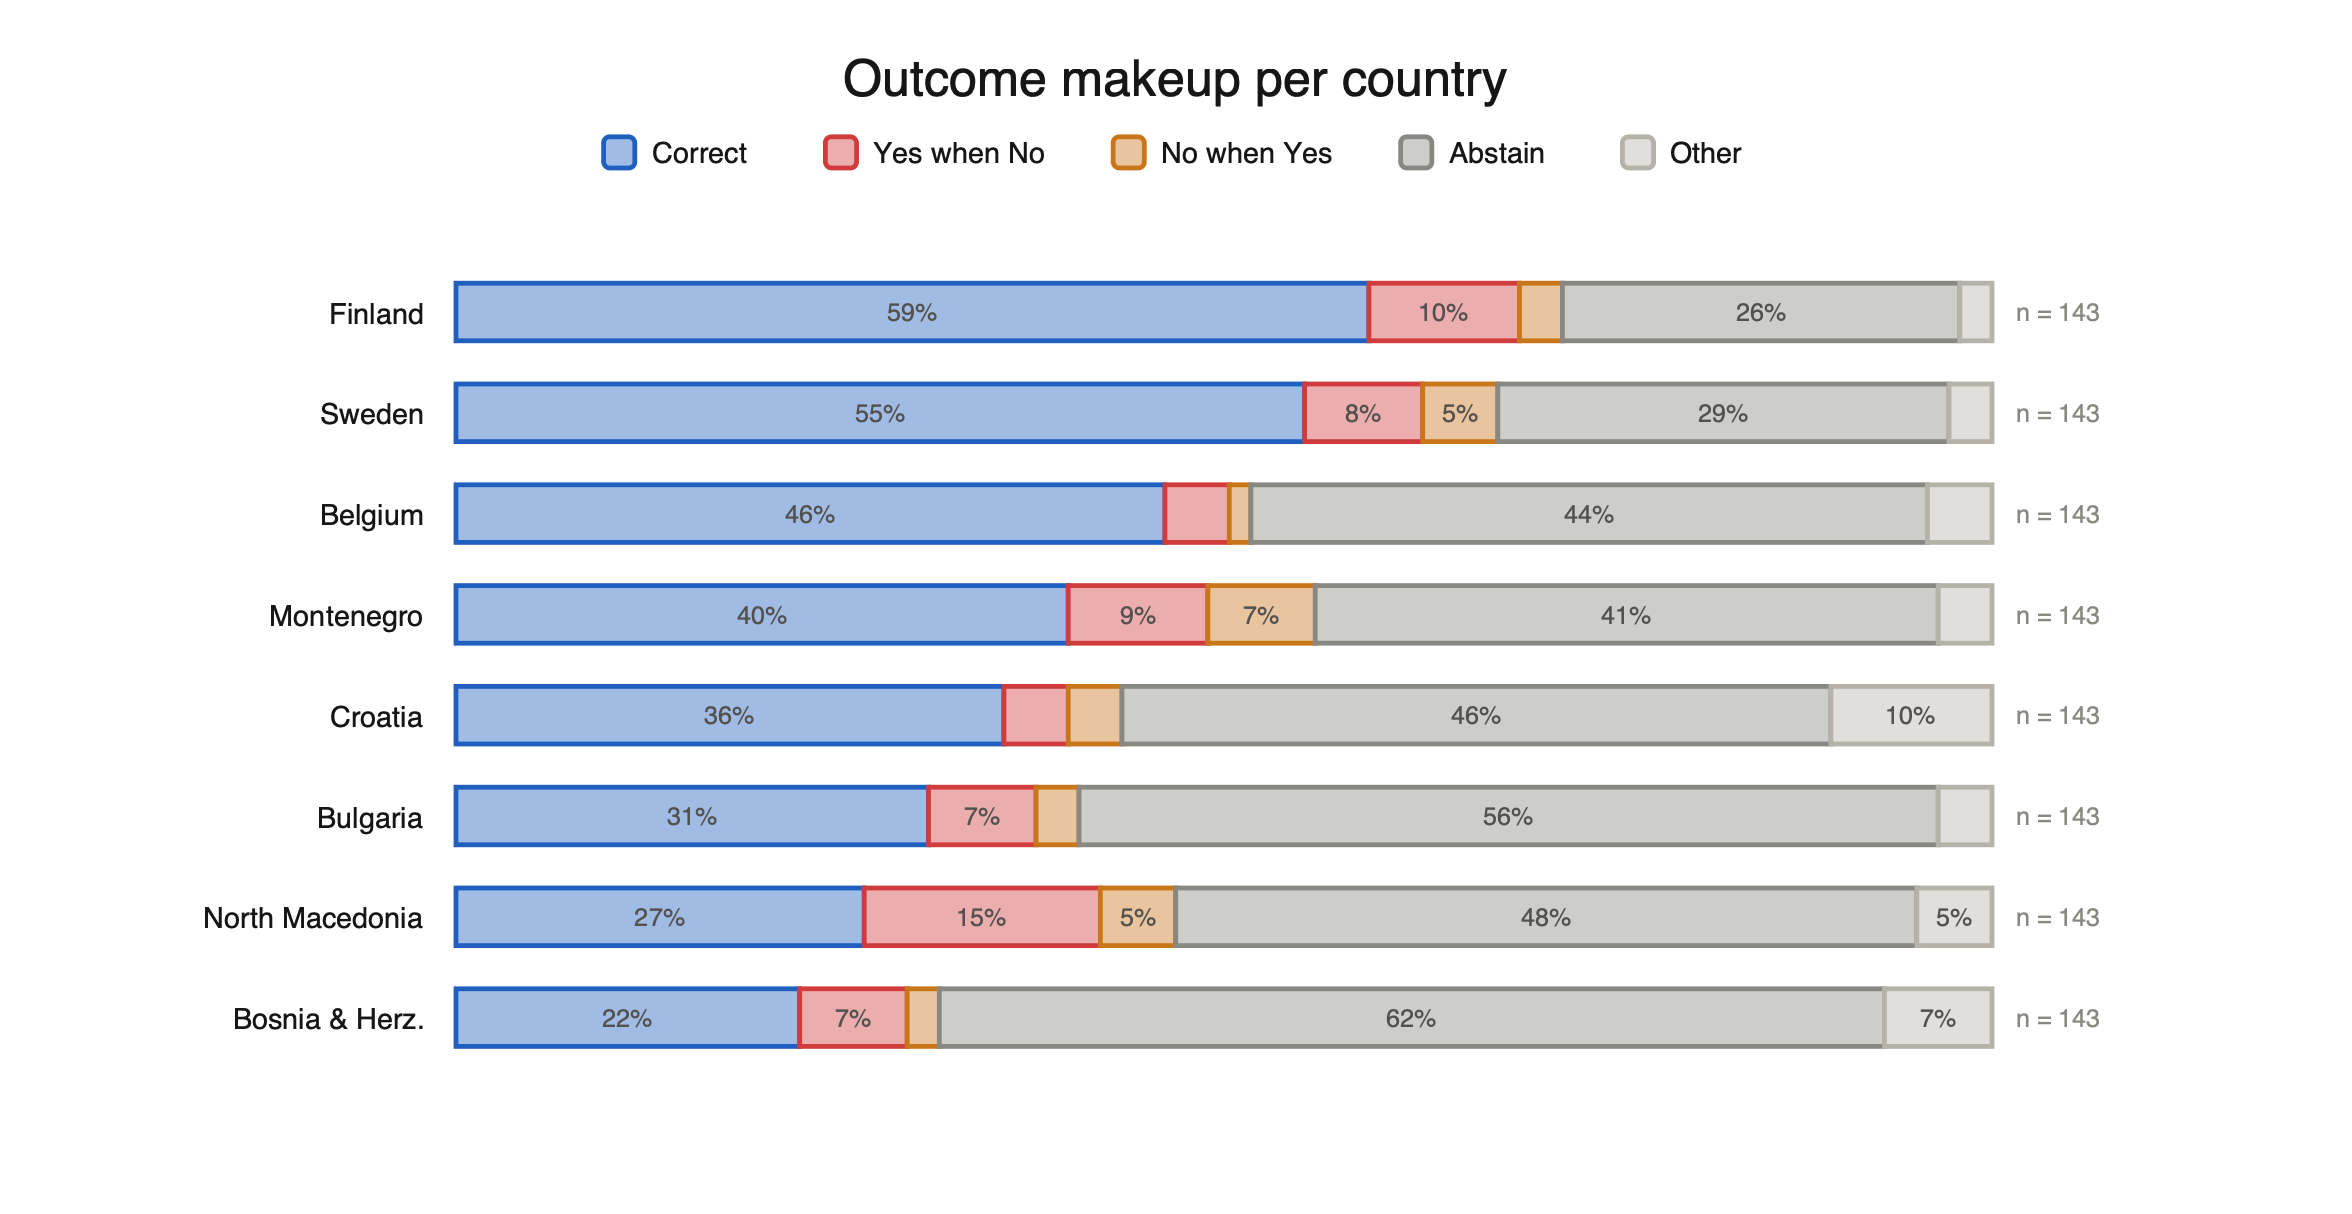
\includegraphics[width=\linewidth]{figures/outcome_makeup_per_country.png}
\caption{Outcome make-up per country.}
\label{fig:outcome-makeup}
\end{figure}

\begin{longtable}[]{@{}
  >{\raggedright\arraybackslash}p{(\linewidth - 10\tabcolsep) * \real{0.2549}}
  >{\raggedright\arraybackslash}p{(\linewidth - 10\tabcolsep) * \real{0.1471}}
  >{\raggedright\arraybackslash}p{(\linewidth - 10\tabcolsep) * \real{0.1471}}
  >{\raggedright\arraybackslash}p{(\linewidth - 10\tabcolsep) * \real{0.1471}}
  >{\raggedright\arraybackslash}p{(\linewidth - 10\tabcolsep) * \real{0.1471}}
  >{\raggedright\arraybackslash}p{(\linewidth - 10\tabcolsep) * \real{0.1569}}@{}}
\caption{The evaluation run read four ways. Coverage is over all 1,144 pairs. The accuracy columns are over the 907 whose published answer is a plain yes or no. Every rate carries its own denominator, and the forced and closed-book rows score an abstention as a miss.}\label{tab:four-ways}\\
\toprule\noalign{}
\begin{minipage}[b]{\linewidth}\raggedright
\textbf{Reading}
\end{minipage} & \begin{minipage}[b]{\linewidth}\raggedright
\textbf{Coverage}
\end{minipage} & \begin{minipage}[b]{\linewidth}\raggedright
\textbf{Accuracy}
\end{minipage} & \begin{minipage}[b]{\linewidth}\raggedright
\textbf{Yes golds}
\end{minipage} & \begin{minipage}[b]{\linewidth}\raggedright
\textbf{No golds}
\end{minipage} & \begin{minipage}[b]{\linewidth}\raggedright
\textbf{Balanced}
\end{minipage} \\
\midrule\noalign{}
\endfirsthead
\toprule\noalign{}
\begin{minipage}[b]{\linewidth}\raggedright
\textbf{Reading}
\end{minipage} & \begin{minipage}[b]{\linewidth}\raggedright
\textbf{Coverage}
\end{minipage} & \begin{minipage}[b]{\linewidth}\raggedright
\textbf{Accuracy}
\end{minipage} & \begin{minipage}[b]{\linewidth}\raggedright
\textbf{Yes golds}
\end{minipage} & \begin{minipage}[b]{\linewidth}\raggedright
\textbf{No golds}
\end{minipage} & \begin{minipage}[b]{\linewidth}\raggedright
\textbf{Balanced}
\end{minipage} \\
\midrule\noalign{}
\endhead
\bottomrule\noalign{}
\endlastfoot
Aggregate Accuracy & 100\% & \begin{minipage}[t]{\linewidth}\raggedright
42.4\%\\
385/907\strut
\end{minipage} & \begin{minipage}[t]{\linewidth}\raggedright
54.7\%\\
295/539\strut
\end{minipage} & \begin{minipage}[t]{\linewidth}\raggedright
24.5\%\\
90/368\strut
\end{minipage} & 39.6\% \\
Commit Accuracy & \begin{minipage}[t]{\linewidth}\raggedright
55.6\%\\
636/1,144\strut
\end{minipage} & \begin{minipage}[t]{\linewidth}\raggedright
70.1\%\\
437/623\strut
\end{minipage} & \begin{minipage}[t]{\linewidth}\raggedright
87.0\%\\
295/339\strut
\end{minipage} & \begin{minipage}[t]{\linewidth}\raggedright
48.9\%\\
90/184\strut
\end{minipage} & 68.0\% \\
Closed book, retrieval off & 75.6\%865/1,144 & \begin{minipage}[t]{\linewidth}\raggedright
43.0\%\\
390/907\strut
\end{minipage} & \begin{minipage}[t]{\linewidth}\raggedright
43.6\%\\
235/539\strut
\end{minipage} & \begin{minipage}[t]{\linewidth}\raggedright
42.1\%\\
155/368\strut
\end{minipage} & 42.9\% \\
Always-yes baseline & 100\% & \begin{minipage}[t]{\linewidth}\raggedright
59.4\%\\
539/907\strut
\end{minipage} & 100\% & 0\% & 50.0\% \\
\end{longtable}

The swarm was dispatched over all 1,144 question-country pairs of the eight countries. It committed to an answer on 636 and declined the remaining 508, split by country in Figure~\ref{fig:outcome-makeup}, a coverage of 55.6\%. Over just the committed answers it scored an accuracy of 70.1\%. Table~\ref{tab:four-ways} presents the results, distinguishing aggregate accuracy (including abstentions), commit accuracy (excluding abstentions), the accuracy of always answering ``yes'', and the accuracy of using only the model's priors. The table compares the 907 pairs that take a binary answer and carry a plain yes or no in the key. The remaining 237 either ask for a band or a count, where an always-yes baseline has no meaning, or are questions the assessors did not answer ``yes'' or ``no''.


Scoring every abstention as an error gives a strict lower bound. On that reading the swarm reaches 42.4\% accuracy, against the 59.4\% returned by arbitrarily answering ``yes'' to every question. Balanced accuracy, the mean of the yes- and no-recalls, falls to 39.6\%, against the 50.0\% any single-class rule achieves by construction. This reading is not how the system was intended, as many questions do not have sufficient public evidence to answer, and thus abstention is the correct path in these cases, but it establishes that the system has no aggregate advantage over the majority class once abstention is removed.

Section~\ref{sec:llm-limitations} raised the issue of generative models using prior beliefs to steer their information retrieval, and a closed-book run over the same eight countries, with retrieval disabled so that the model answers from its parameters alone, reaches 43.0\% on the same 907 golds. Aggregate accuracy and closed book accuracy are indistinguishable. Retrieval therefore buys no measurable gain once every abstention is counted as a wrong answer. The difference appears in the two classes. Without retrieval the model is close to symmetric, recovering 43.6\% of yes golds and 42.1\% of no golds. With retrieval the swarm recovers 87.0\% and 48.9\%. What the pipeline finds settles a positive claim and does little for a negative one, which is the asymmetry Section~\ref{sec:llm-limitations} predicted and the remainder of this chapter returns to.



\begin{figure}[htbp]
\centering
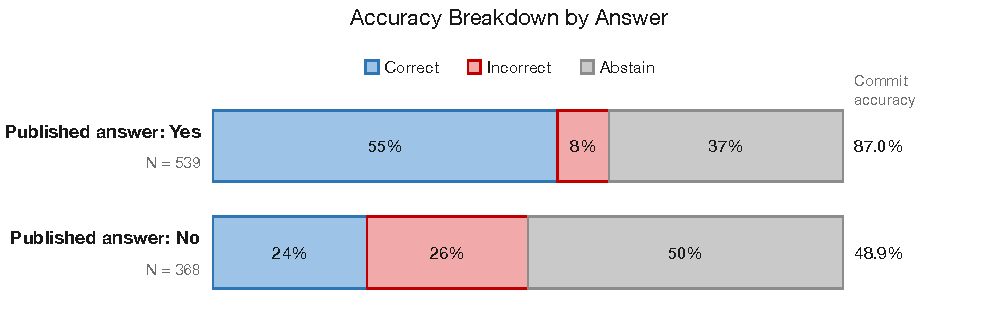
\includegraphics[width=\linewidth]{figures/fig_4_1_yes_no.pdf}
\caption{Decomposition of accuracy by answer class.}
\label{fig:accuracy-by-class}
\end{figure}

Accuracy divides unevenly between the two answer classes. Where the published key records a ``yes'', the swarm committed on 339 of 539 pairs and agreed with the key on 87.0\% of them. Where the key records a ``no'', it committed on 184 of 368 and agreed on 48.9\%, so on the negative golds it commits to, it is wrong more often than right. Abstention divides the same way, as Figure~\ref{fig:accuracy-by-class} shows. The swarm declines exactly half the negative golds against 37.1\% of the positive ones. The answer it withholds most often is the one that records a country falling short.

The error the Verifier exists to prevent is a committed ``yes'' against a negative gold. The run contains 91 of them, 24.7\% of all 368 negative golds and 49.5\% of the 184 the swarm was willing to commit on. Offered the choice between declining and asserting a ``yes'' the evidence does not carry, it asserts about half the time.

On the first condition of Convergent Validity the system reaches 70.1\% commit accuracy at 55.6\% coverage. It agrees with the existing process on most of the answers it gives, and it gives an answer to just over half the questions.



\begin{figure}[htbp]
\centering
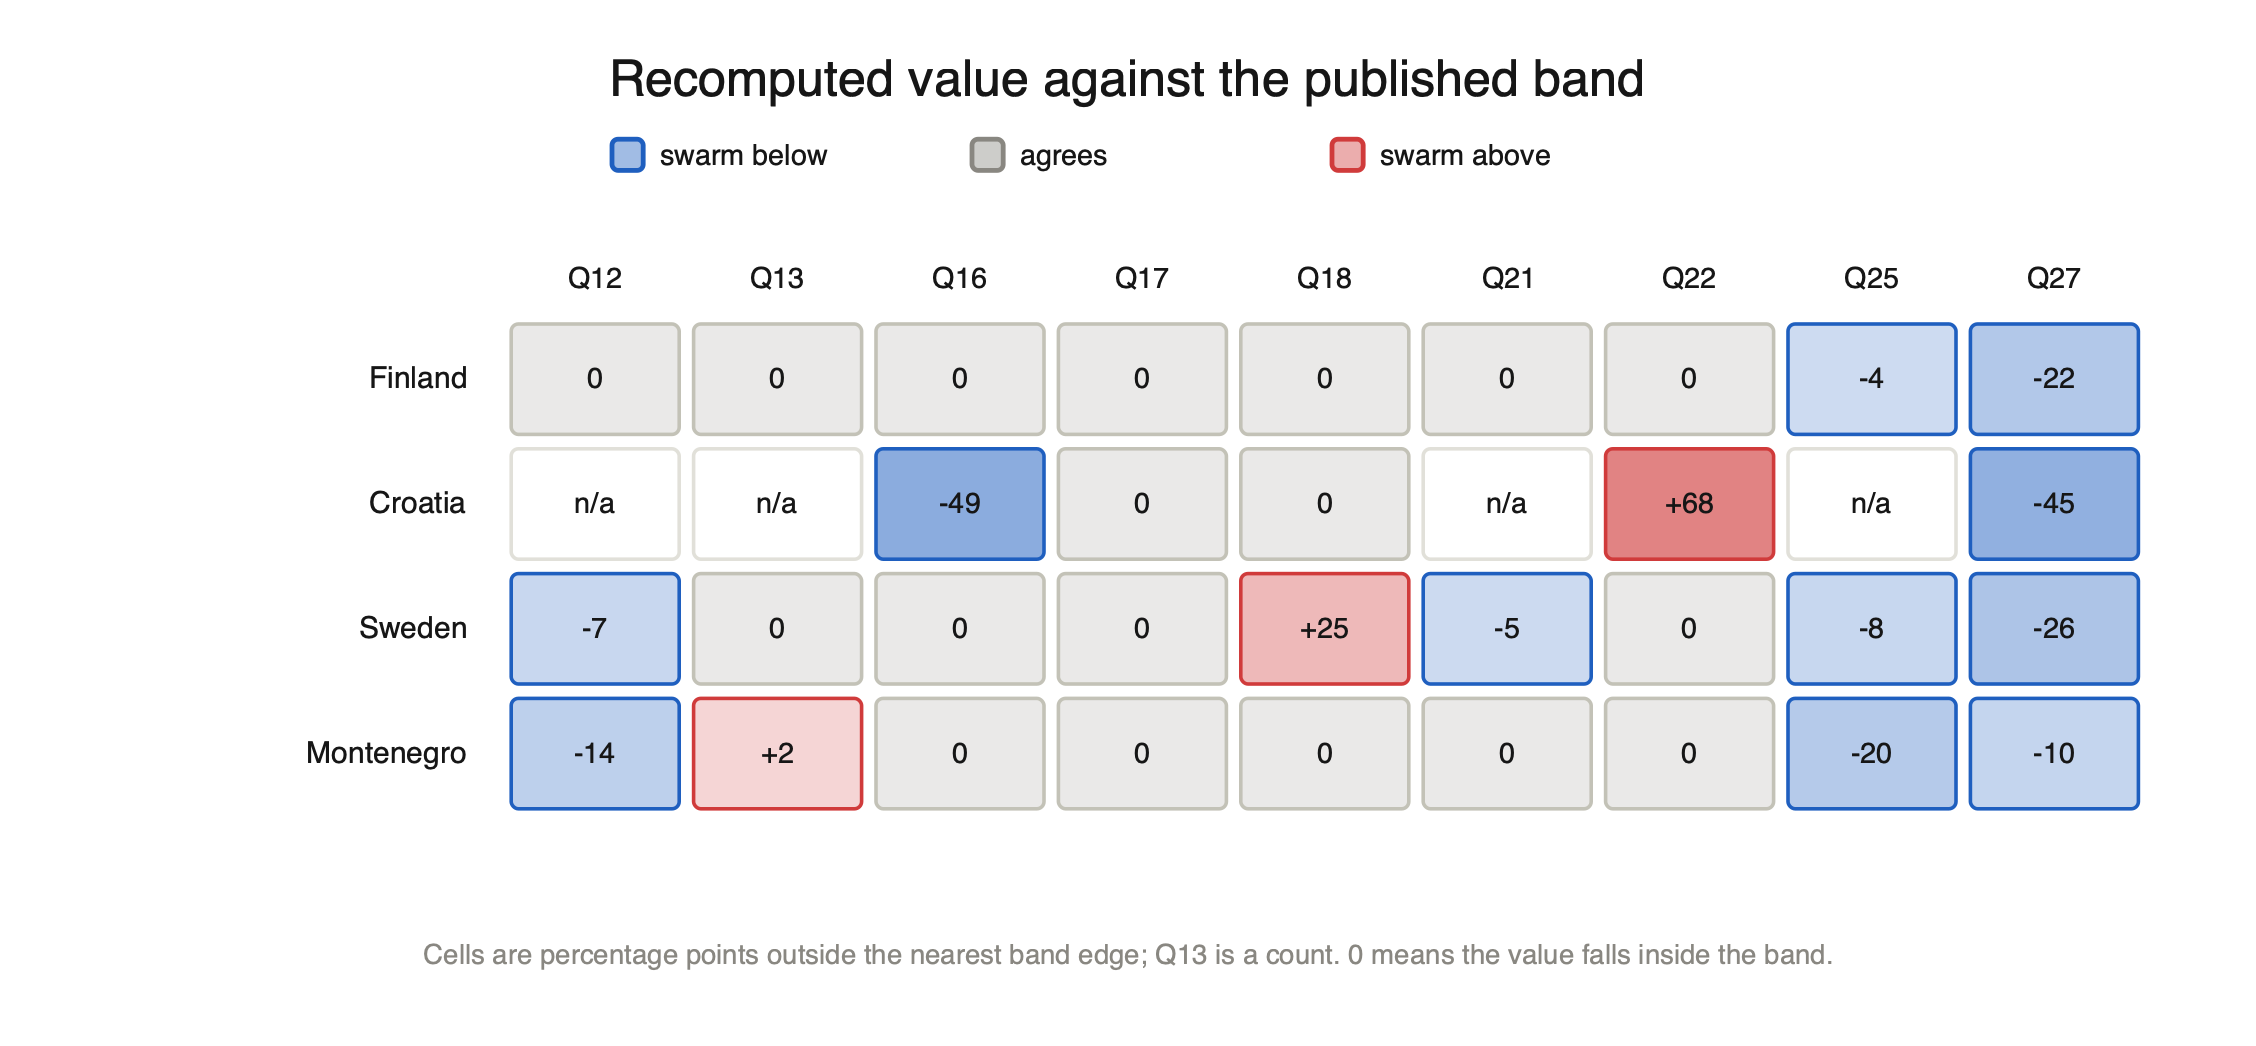
\includegraphics[width=\linewidth]{figures/recompute_vs_band.png}
\caption{Recomputed value against the published band.}
\label{fig:recompute-band}
\end{figure}

Only four of the eight countries (Finland, Croatia, Sweden and Montenegro) had harvestable portals.

Across the thirty-six measurable cells the recompute agrees with the published key on eighteen, 50\% agreement, broken down by country in Figure~\ref{fig:recompute-band}. The disagreements do not all run in the same direction, so this is not a case of countries systematically inflating their score. The figure shows the numbers diverging, with Montenegro\textquotesingle s stated licence coverage exceeding 90\% where the recompute reads 70\%, an overstatement, while Croatia\textquotesingle s published figure for Q22 sits at 10-30\% against a recompute above 90\%, an understatement of what the portal actually carries. This recompute is not infallible, as the Verifier recomputes the scores over the cached data that the Researcher retrieved, and there is no separate route or evidence pool to check against.

Convergent Validity is therefore only half met. The system reproduces the existing process on 70.1\% of the answers it commits to. The recompute tested the harder question, whether the figures a country reports about its own portal survive a check against the portal itself. On these nine they do not. The self-report and an independent count disagree on 50\% of the measurable cells, which is evidence that the reported figures on the objective quality questions are often inaccurate. It falls short of proof, because the recompute has no route independent of the Researcher\textquotesingle s harvest, so no single figure is settled. Capgemini already amends 10\% of the answers countries submit, which is the assessment\textquotesingle s own admission that self-reports are sometimes wrong, and on the small set of questions where an outside check is possible, the recompute points the same ways.

\section{Selectivity}\label{sec:selectivity}

Abstention exists so the swarm does not commit answers with shaky underlying evidence. Table~\ref{tab:abstention-reasons} breaks the 508 abstentions down by reason, and Appendix~\ref{app:pipeline-detail} carries the full trail. Every one passed through the Adjudicator, which returned an abstain verdict on 413; a commit gate withheld a further 82 at the 0.65 floor, and in 13 more the Adjudicator's own answer was inconclusive. No abstention in this run came from an empty search, and a gold answer existed for 94.3\% of these questions.

\begin{longtable}[]{@{}
  >{\raggedright\arraybackslash}p{(\linewidth - 4\tabcolsep) * \real{0.4531}}
  >{\raggedright\arraybackslash}p{(\linewidth - 4\tabcolsep) * \real{0.2031}}
  >{\raggedright\arraybackslash}p{(\linewidth - 4\tabcolsep) * \real{0.3437}}@{}}
\caption{Why the swarm abstained.}\label{tab:abstention-reasons}\\
\toprule\noalign{}
\begin{minipage}[b]{\linewidth}\raggedright
\textbf{Reason for abstaining}
\end{minipage} & \begin{minipage}[b]{\linewidth}\raggedright
\textbf{Pairs}
\end{minipage} & \begin{minipage}[b]{\linewidth}\raggedright
\textbf{Share of abstentions}
\end{minipage} \\
\midrule\noalign{}
\endfirsthead
\toprule\noalign{}
\begin{minipage}[b]{\linewidth}\raggedright
\textbf{Reason for abstaining}
\end{minipage} & \begin{minipage}[b]{\linewidth}\raggedright
\textbf{Pairs}
\end{minipage} & \begin{minipage}[b]{\linewidth}\raggedright
\textbf{Share of abstentions}
\end{minipage} \\
\midrule\noalign{}
\endhead
\bottomrule\noalign{}
\endlastfoot
Verifier rejected the evidence & 208 & 40.9\% \\
Researcher never reached the floor & 199 & 39.2\% \\
Researcher never committed & 30 & 5.9\% \\
Quote absent from retrieved pages & 24 & 4.7\% \\
Instrumentation mismatch & 19 & 3.7\% \\
Fetch error & 16 & 3.1\% \\
Blocked by the deny-list & 12 & 2.4\% \\
All abstentions & 508 & 100.0\% \\
\end{longtable}


Section~\ref{sec:open-world} highlighted how moving the evidence pool from self-reporting to the open web means absence of evidence of a practice no longer equates to absence of the practice itself. Question PT28 asks, ``Do you monitor search key words?''. It is easier to find evidence when the national data team do follow a practice, since they may have posted on their portal that they do. For the swarm to mark it ``no'' with confidence, it must find concrete evidence that they do not, and a national data team is unlikely to publish that it is not following a practice. Accordingly, 19 of the 143 questions were abstained on by at least 7 countries, and 12 of these covered internal practices. Any evidence the swarm finds may be related to the practice without directly addressing it, so it will be less confident in these answers. This is reflected in the results: across all answer shapes the swarm abstains on 50.0\% of no golds against 37.1\% of yes golds.

Figure~\ref{fig:per-class-confidence} sweeps the confidence threshold required to commit an answer from 0.40 upwards and rescores the gold classes on what survives at each setting. The two classes diverge as the threshold increases. On yes golds the threshold acts as expected, with accuracy climbing from 87.0\% at the 0.65 floor and reaching 100\% near 0.95, on nine answers. On no golds it moves the other way, falling from 48.9\% at the floor to zero by about 0.81 and staying there.\textbf{ }



\begin{figure}[htbp]
\centering
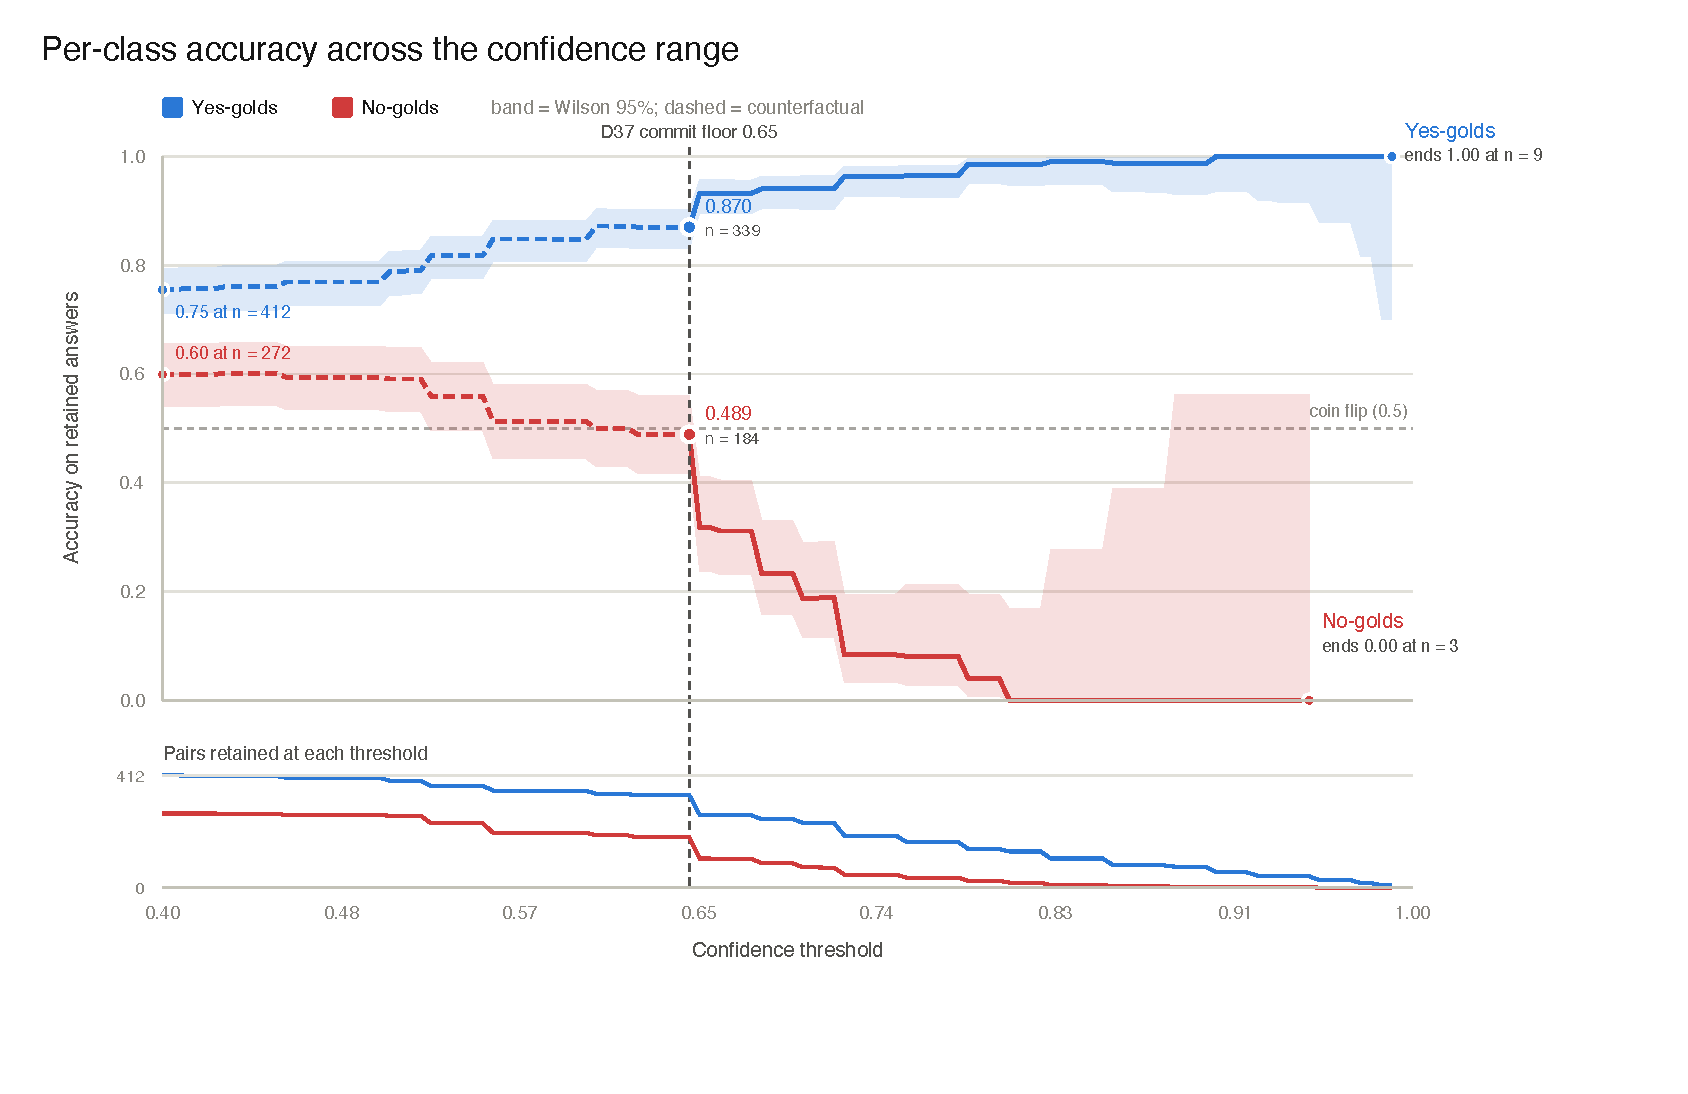
\includegraphics[width=\linewidth]{figures/per_class_accuracy_full_range.pdf}
\caption{Per-class accuracy across the confidence range.}
\label{fig:per-class-confidence}
\end{figure}

Calibration shows the same inversion. A stated confidence of 0.8 should correspond to being right about 80\% of the time. Across all 623 scoreable committed answers the expected calibration error is 0.063, which taken alone reads as a well-calibrated system. Figure~\ref{fig:reliability} shows otherwise. On the yes golds every point sits on or above the diagonal, so the system is modestly under-confident, which is a more harmless direction in which to err. On the no golds the sequence runs backwards and the expected calibration error is 0.299, nearly five times the aggregate. The aggregate conceals this because the classes are unevenly spread across the range, with only 3 negative samples in the uppermost bin against 77 yes golds. Because nothing commits below 0.65, six of the ten pre-registered bins are empty and calibration is observable only across the upper third of the scale.



\begin{figure}[htbp]
\centering
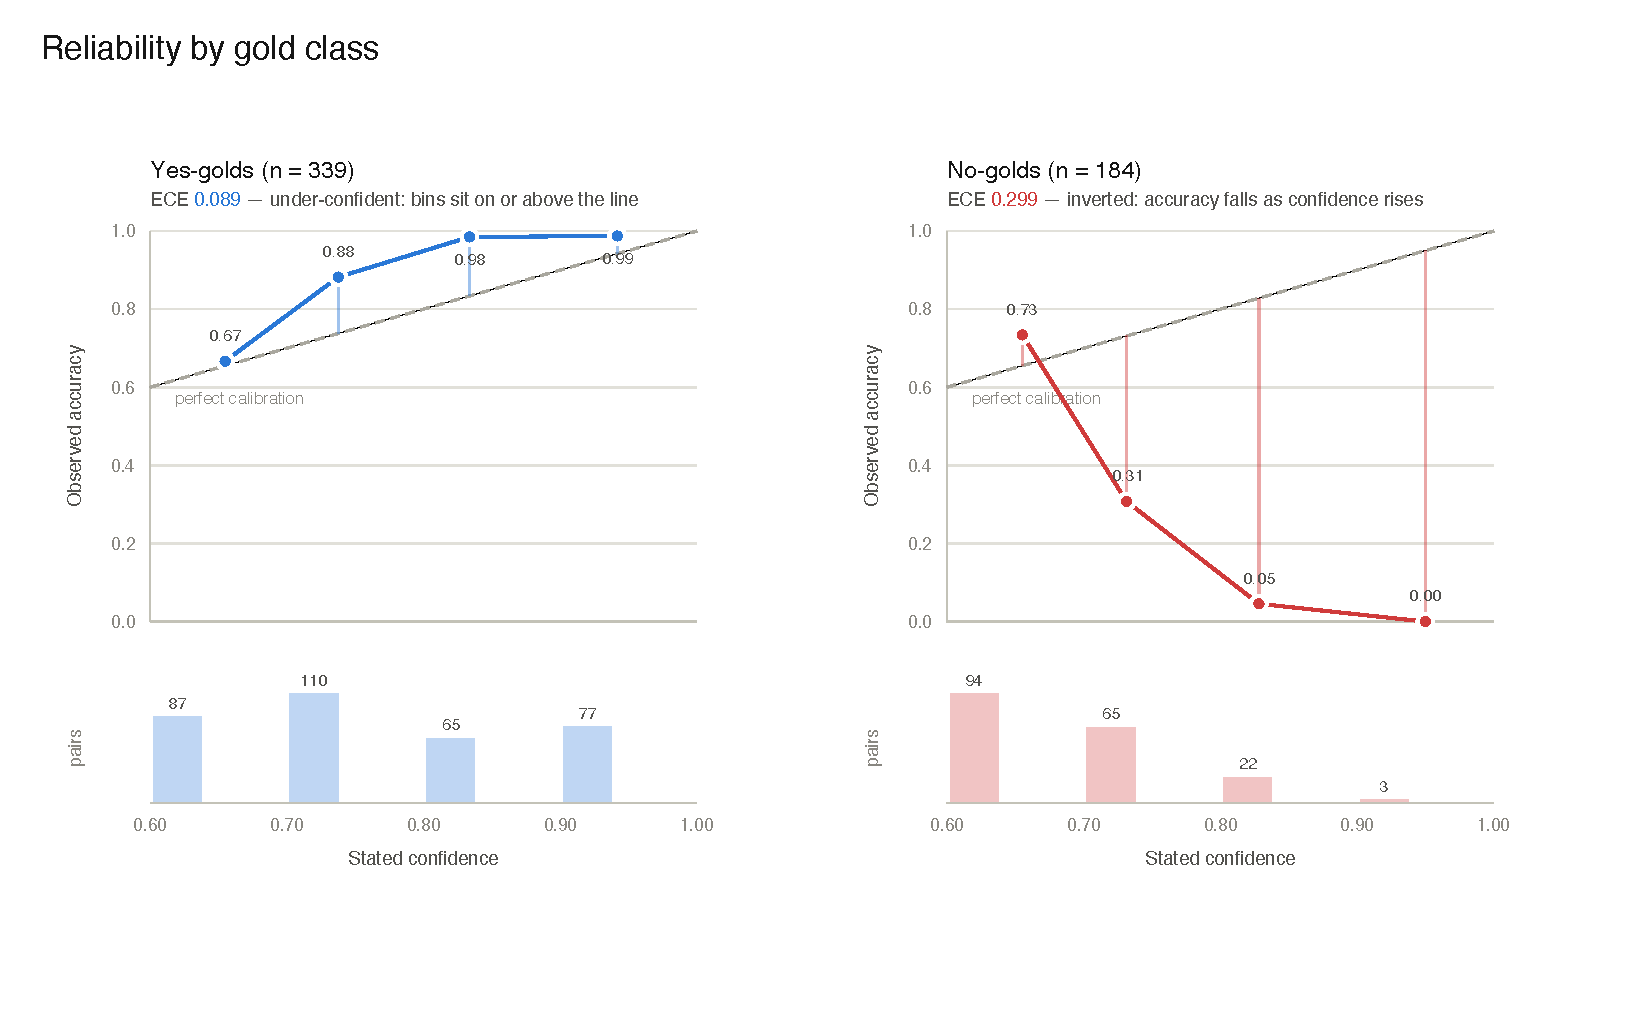
\includegraphics[width=\linewidth]{figures/reliability_by_class.pdf}
\caption{Reliability by gold class.}
\label{fig:reliability}
\end{figure}

The inversion continues below the floor. The dashed segment of Figure~\ref{fig:per-class-confidence} scores answers the swarm produced and then withheld, all from pairs where the Researcher never reached 0.65 on any attempt. Of the 162 that are scoreable, 73 carry a yes gold and 89 carry a no gold. Around a quarter of the yes answers are correct, against 79 of the 89 no answers. The negatives the system is least sure of are the ones it gets right, and the same holds just above the floor, where the 0.65 to 0.70 group is correct 73\% of the time. When the swarm cannot find evidence for a question, which is what would constitute a ``no'' under a closed-world assumption, it outputs a low confidence score because any evidence it did retrieve was weak. The information is therefore present in the score and cannot be used, because these correct ``noes'' look the same as the incorrect ``yesses'', so there can be no separation before looking at the key. There are also far more ``yesses'' than ``noes'' in the answer key, so optimising the threshold on raw accuracy would favour maximising the chance of getting a ``yes'' correct, losing many correct ``noes'' with them.

Selectivity as implemented meets the first of Section~\ref{sec:criteria}'s two requirements and fails the second. The system does decline, on 44\% of pairs. The confidence attached to an answer measures how strongly the retrieved passage supports it, not how likely it is to be right, and thus negative golds, which hold little public evidence, frequently fall below the confidence floor. The system is well-calibrated for answering ``yes'', but systemically disadvantaged for answering ``no''.

\section{Attributability}\label{sec:attributability}

Attributability was defined in Section~\ref{sec:criteria} by two conditions. The quoted passage must exist in the source, and a reasonable reader must agree it supports the claim. The first is a string comparison the system enforces on every answer before it commits; the second needs a reader, and Section~\ref{sec:agent-loop} puts the Verifier in charge of this role. Attributability's value is that an assessed country knows its score rests on well-evidenced grounds, and can contest the evidence held against it.

The first condition is enforced mechanically. The offline gate described in Section~\ref{sec:agent-loop} compares the Researcher\textquotesingle s quoted passage against the snippets it read and fails the answer where the passage does not appear. It sits upstream of the commit decision, so all 636 committed answers passed it, and 24 of the run\textquotesingle s 508 abstentions record an ungrounded passage as the reason. Fabrication, one of the central risks of a generative assessor identified in Section~\ref{sec:llm-limitations}, is caught by a string comparison and is not what limits the system.

Testing for misinterpretation requires a `reasonable reader'. The Verifier\textquotesingle s role is to apply the scrutiny a human reader would bring to the submitted evidence. Table~\ref{tab:attributability} displays the 208 relevance rejections, which are pairs where the quote survived the string comparison and the Verifier ruled the evidence off-target anyway, so off-target evidence outnumbers absent evidence by more than eight to one.

\begin{longtable}[]{@{}
  >{\raggedright\arraybackslash}p{(\linewidth - 6\tabcolsep) * \real{0.3750}}
  >{\raggedright\arraybackslash}p{(\linewidth - 6\tabcolsep) * \real{0.3409}}
  >{\raggedright\arraybackslash}p{(\linewidth - 6\tabcolsep) * \real{0.1136}}
  >{\raggedright\arraybackslash}p{(\linewidth - 6\tabcolsep) * \real{0.1705}}@{}}
\caption{What each attributability condition caught, over the 1,144 evaluation pairs.}\label{tab:attributability}\\
\toprule\noalign{}
\begin{minipage}[b]{\linewidth}\raggedright
\textbf{Attributability condition}
\end{minipage} & \begin{minipage}[b]{\linewidth}\raggedright
\textbf{What fails it}
\end{minipage} & \begin{minipage}[b]{\linewidth}\raggedright
\textbf{Pairs}
\end{minipage} & \begin{minipage}[b]{\linewidth}\raggedright
\textbf{Share of 1,144}
\end{minipage} \\
\midrule\noalign{}
\endfirsthead
\toprule\noalign{}
\begin{minipage}[b]{\linewidth}\raggedright
\textbf{Attributability condition}
\end{minipage} & \begin{minipage}[b]{\linewidth}\raggedright
\textbf{What fails it}
\end{minipage} & \begin{minipage}[b]{\linewidth}\raggedright
\textbf{Pairs}
\end{minipage} & \begin{minipage}[b]{\linewidth}\raggedright
\textbf{Share of 1,144}
\end{minipage} \\
\midrule\noalign{}
\endhead
\bottomrule\noalign{}
\endlastfoot
The passage exists in the cited source & quote absent from the retrieved text & 24 & 2.1\% \\
A reader agrees it supports the claim & Verifier ruled the evidence off-target & 208 & 18.2\% \\
Both conditions cleared & answer committed & 636 & 55.6\% \\
Neither condition reached & abstained for another reason & 276 & 24.1\% \\
\end{longtable}


Scrutiny of the Researcher's claims from the Verifier raises the commit rate from 26.6\% to 46\% and the correct answers from 220 to 372 (Section~\ref{sec:ablation}). It converts 165 of the Researcher\textquotesingle s wrong or withheld answers into correct ones and loses 13 in the other direction, moving 178 answers in all. The Adjudicator improves upon this by committing an extra 110 answers and getting 65 right, and it overturns none of the Verifier\textquotesingle s existing decisions. This is the extent to which the architecture can ensure a `reasonable' reader is judging that claims are valid without an external model or human verification layer, and the Adjudicator correcting zero of the Verifier's claims hints that each reasoning stage converges closer to the true accuracy ceiling.

Opus 4.6 reviewed the 91 cases where the swarm committed a ``yes'' against a negative gold, with both the swarm\textquotesingle s evidence and the ODMI\textquotesingle s explanation in front of it, to test whether the swarm had misattributed its evidence or the published answer was wrong or out of date. On 84 of the 91 it judged the cited passage simply too weak to carry the claim. On the other seven it found the evidence sufficient and the published ``no'' defensible or out of date, and four of those seven carry no published explanation at all. Opus shares a training lineage with the Sonnet agents, so a stronger test is another model family or a human reader. What this small experiment confirmed is that misattribution is a failure mode of the swarm, rather than the answer key being consistently incorrect.

636 committed answers cleared the string comparison and 24 abstentions record a quote that did not, which settles the first condition. The Verifier performs the role of the reasonable reader well, halting 208 of the Researcher\textquotesingle s overreaching claims, but still lets through 91, showing the issue is not solved. In production, where there is no answer key to check against, the many overreads that slip through the system will remain undetected, and this is where an external model or human reviewer would be valuable.

\section{Subgroup Equity}\label{sec:subgroup-equity}

Subgroup Equity asks whether the same standard of assessment applied to every country. This section analyses which properties are incidental to maturity and which are inseparable from it, because only the first kind can be removed. The evaluation set was stratified to test the clearest incidental candidate, language comprehension. Section~\ref{sec:multilingual} set out three explanations for a poor score: the model misreads evidence written in the national language, the evidence is not published at all, or the country is truly less open. The two strata separate the first of these from the other two, with stratum A holding the four lower-resource languages (Bosnia and Herzegovina, North Macedonia, Montenegro and Bulgaria) and stratum B the four higher-resource ones (Finland, Croatia, Sweden and Belgium).

\begin{longtable}[]{@{}
  >{\raggedright\arraybackslash}p{(\linewidth - 10\tabcolsep) * \real{0.2059}}
  >{\raggedright\arraybackslash}p{(\linewidth - 10\tabcolsep) * \real{0.0882}}
  >{\raggedright\arraybackslash}p{(\linewidth - 10\tabcolsep) * \real{0.1275}}
  >{\raggedright\arraybackslash}p{(\linewidth - 10\tabcolsep) * \real{0.1863}}
  >{\raggedright\arraybackslash}p{(\linewidth - 10\tabcolsep) * \real{0.1863}}
  >{\raggedright\arraybackslash}p{(\linewidth - 10\tabcolsep) * \real{0.2059}}@{}}
\caption{Outcomes by resource stratum.}\label{tab:strata}\\
\toprule\noalign{}
\begin{minipage}[b]{\linewidth}\raggedright
\textbf{Stratum}
\end{minipage} & \begin{minipage}[b]{\linewidth}\raggedright
\textbf{Pairs}
\end{minipage} & \begin{minipage}[b]{\linewidth}\raggedright
\textbf{Abstention}
\end{minipage} & \begin{minipage}[b]{\linewidth}\raggedright
\textbf{Commit accuracy}
\end{minipage} & \begin{minipage}[b]{\linewidth}\raggedright
\textbf{Neg-gold FP (all)}
\end{minipage} & \begin{minipage}[b]{\linewidth}\raggedright
\textbf{Neg-gold FP (committed)}
\end{minipage} \\
\midrule\noalign{}
\endfirsthead
\toprule\noalign{}
\begin{minipage}[b]{\linewidth}\raggedright
\textbf{Stratum}
\end{minipage} & \begin{minipage}[b]{\linewidth}\raggedright
\textbf{Pairs}
\end{minipage} & \begin{minipage}[b]{\linewidth}\raggedright
\textbf{Abstention}
\end{minipage} & \begin{minipage}[b]{\linewidth}\raggedright
\textbf{Commit accuracy}
\end{minipage} & \begin{minipage}[b]{\linewidth}\raggedright
\textbf{Neg-gold FP (all)}
\end{minipage} & \begin{minipage}[b]{\linewidth}\raggedright
\textbf{Neg-gold FP (committed)}
\end{minipage} \\
\midrule\noalign{}
\endhead
\bottomrule\noalign{}
\endlastfoot
Stratum A (lower resource) & 572 & 52.3\% & 61.1\% (162/265) & 21.1\% (55/261) & 42.6\% (55/129) \\
Stratum B (higher) & 572 & 36.5\% & 76.8\% (275/358) & 33.6\% (36/107) & 65.5\% (36/55) \\
\end{longtable}


Stratum A has over double the negative-golds of B, and would be expected to perform worse as Section~\ref{sec:convergent-validity} found the swarm handles ``yesses'' far better than ``noes''. However, stratum A\textquotesingle s negative gold false positive rate is far lower than B\textquotesingle s in both aggregate and commit-only, at 0.211 against 0.336 in aggregate and 0.426 against 0.655 on committed negatives. The obvious objection is that stratum A simply declines more of the hard negatives. That does not hold, since the swarm abstains on 50.6\% of negative golds in stratum A against 48.6\% in stratum B. Weaker language comprehension did not produce confident error.

Table~\ref{tab:strata} shows that what rises in stratum A is abstention, at 52.3\% against stratum B\textquotesingle s 36.5\%, and commit accuracy is lower, at 61.1\% against 76.8\%. That appears to contradict the false-positive result, since a stratum with lower accuracy might be expected to make more of every kind of error. The two measures cover different populations. Commit accuracy covers every committed answer of either class, while the false-positive rate covers only negative golds, of which stratum A had many more. So the aggregate figure reflects the class imbalance between the strata, with stratum B performing better overall, despite being much worse on the few negative answers it held.

The 15.7\% abstention gap can be traced back to what triggered it in the pipeline. Stratum A abstains on 299 of its 572 pairs against stratum B\textquotesingle s 209, and around 96\% of that gap sits at the Researcher\textquotesingle s confidence landing below the threshold. This happened on 143 pairs in stratum A against 56 in stratum B. The Verifier\textquotesingle s own relevance rejections are marginally more common in the higher-resource group at 107 against 101. Fetch failures run at sixteen in stratum A against none in stratum B, fourteen of them in Bulgaria alone, which is small and one-sided. The stratum difference therefore moves how confident the Researcher is in what it read, and leaves untouched how the Verifier judges whether that evidence is on target. The Researcher is struggling to find any good evidence in the first place, and states so immediately. What stays unseparated is whether a low confidence score in stratum A reflects the model reading the national language less well or the estate publishing less to read, and Section~\ref{sec:reformulation} records that. The stratum is not the dominant axis in any case, since the false-positive rate varies more within each group than between them, spanning 0.128 to 0.301 inside stratum A and 0.222 to 0.483 inside stratum B against a gap of 0.125 between the two.



 

\begin{figure}[htbp]
\centering
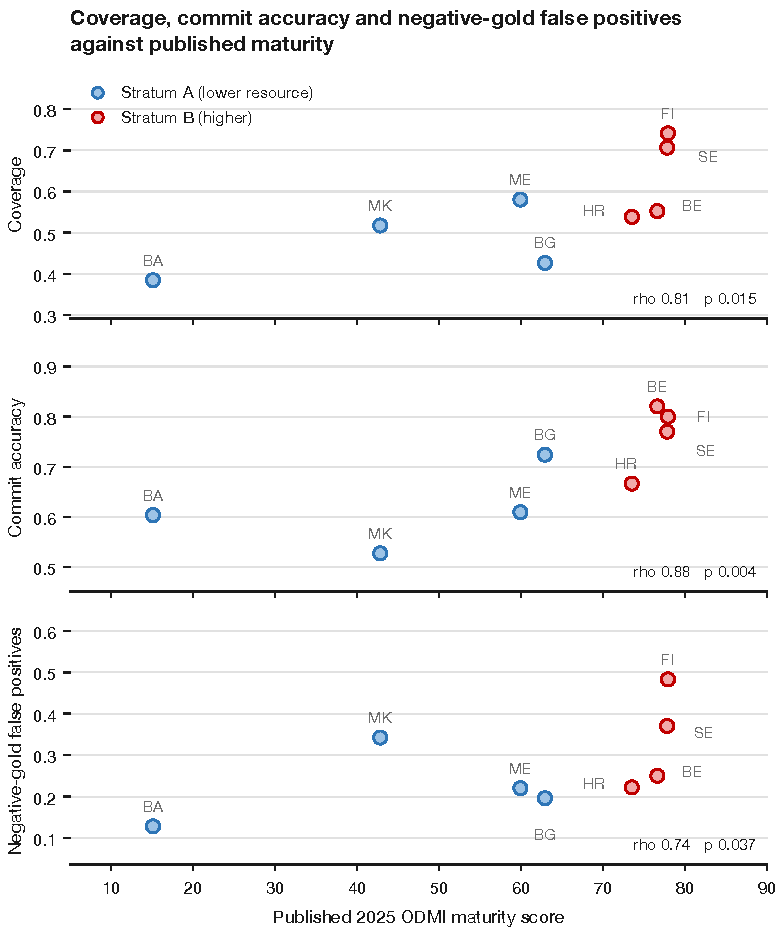
\includegraphics[width=0.72\linewidth]{figures/fig_4_5_maturity.pdf}
\caption{Coverage, commit accuracy and negative-gold false positives against published maturity.}
\label{fig:against-maturity}
\end{figure}

Finland records the highest false-positive rate of the eight countries, at 48.3\%, and Bosnia and Herzegovina the lowest, at 12.8\%, against published maturities of 77.9 and 15.1. Figure~\ref{fig:against-maturity} ranks every country with its published maturity, against coverage, commit accuracy and the false-positive rate, and all three climb with it, at Spearman correlations of 0.81, 0.88 and 0.74. North Macedonia is the exception, at 30.1\% on a maturity of 42.8, above four countries that score higher. The country figures rest on small counts at the mature end, where Belgium holds 24 negative golds and Finland 29, so the ordering is a tendency across the range rather than a difference between any two countries. The rate plotted here divides by every negative gold, including the ones the swarm declined, so a country that abstains more posts a lower one. Measured only on the negative golds it committed to, the correlation with maturity rises to 0.90. One explanation fits, though the present design cannot confirm it.

In mature countries, a negative gold rarely signifies a simple absence. Because such countries implement most practices, a recorded ``no'' is often accompanied by adjacent evidence, partial implementation, a related practice, or a published intention yet to be realised. This near-miss evidence is plentiful and can be interpreted as support for a positive answer. By contrast, in less mature countries a negative gold more commonly indicates a practice that is absent, and the open web yields little that could be confused with it, as they have a sparser web-presence. Section~\ref{sec:llm-limitations} outlines the mechanism by which adjacent evidence leads to over-reading. The denser the evidence base, the more material there is to over-read.

Section~\ref{sec:criteria} set out the requirement that a country\textquotesingle s result depends "solely on its capability in the specific quality that is being assessed". A distinction has to be made. Subgroup Equity requires that a country\textquotesingle s score tracks its maturity alone, whereas here, the swarm\textquotesingle s performance tracks maturity too. Subgroup Equity therefore is not met, and the reason sits in the current form of the assessment. The system recovers 87.0\% of the yes golds it commits to against 48.9\% of the no golds. A country\textquotesingle s maturity is calculated directly from how many answers are negative, so the class the system handles worst makes up a larger part of a low-maturity country\textquotesingle s assessment. A score is built from counts of awarded marks. Stratum A accrues 55 wrongly credited answers against stratum B\textquotesingle s 36, even though its rate per negative gold is the lower of the two. Coverage falls as maturity falls, which is the top panel of Figure~\ref{fig:against-maturity}. Among the answers that do commit, wrong yesses outnumber wrong noes by roughly two to one, so what survives leans towards crediting practices that are not there. Both effects track the country\textquotesingle s position on the scale the index exists to measure, which makes the error a function of the quantity the system intends to measure.

\section{Generalisability}\label{sec:generalisability}

Generalisability asks whether the system performs evenly across the question types and dimensions in the assessment, or whether it has weak points hidden by an aggregated accuracy figure. In the closest published analogue to this work, \textcite{fumega2026} set deep research agents to find evidence on the open web and answer a data-policy questionnaire from it. Their mismatch against the human answers runs from 19\% on the indicator whose evidence sits in a single document to 69\% on the one whose evidence is scattered, averaging 42\% across four indicators. The pooled commit-accuracy in Section~\ref{sec:convergent-validity}, 70.1\% over the 623 committed answers that carry a score, is the kind of figure that invites this question. The headline is therefore broken apart two ways: by ODMI dimension, and by the answer shape each question demands. 

\begin{figure}[htbp]
\centering
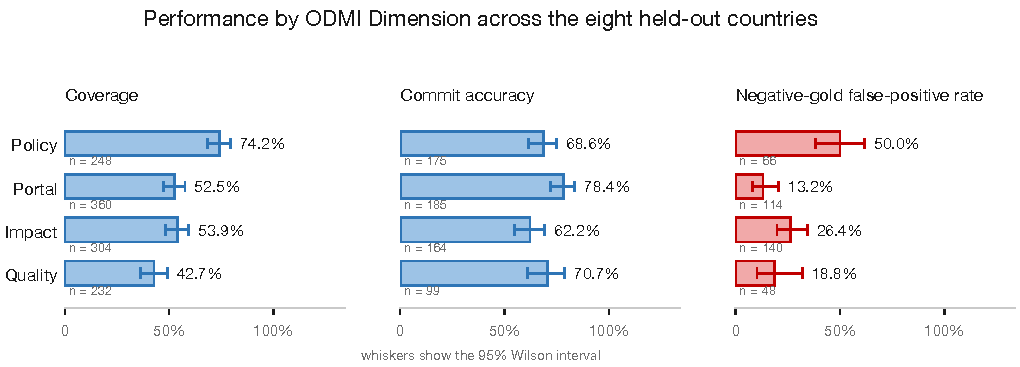
\includegraphics[width=\linewidth]{figures/fig_4_5_dimension.pdf}
\caption{The headline by dimension.}
\label{fig:by-dimension}
\end{figure}

Across the four dimensions the headline holds unevenly, as Figure~\ref{fig:by-dimension} sets out. Commit-accuracy runs from 78.4\% on Portal to 62.2\% on Impact, and coverage varies more, from 74.2\% on Policy to 42.7\% on Quality. Counting abstentions as failures the dimensions sit between 30.2\% for Quality and 48.4\% for Policy. The gap is largest on negative golds, with the false-positive rate at 13.2\% on Portal and 50.0\% on Policy.

Dimension and answer shape are not independent. The graded questions sit almost entirely in Quality, and the nine catalogue questions are most of why the dimension looks unreachable. The 50\% accuracy of the nine questions pull down the rest of the dimension, and once they are set aside the swarm answers Quality at 80.3\% when it commits, so the 70.7\% in Figure~\ref{fig:by-dimension} is the catalogue questions pulling the score down. Quality\textquotesingle s low coverage is the system declining what it cannot ground, which is also why its negative-gold false-positive rate is the second lowest of the four. Portal sits at the other extreme, strongest on both accuracy and false positives, because a portal\textquotesingle s features can be read straight off the portal, the one place where absence of proof does equate to absence of existence. Policy is the revealing case, it answers the most and gets half of its negative golds wrong.



\begin{figure}[htbp]
\centering
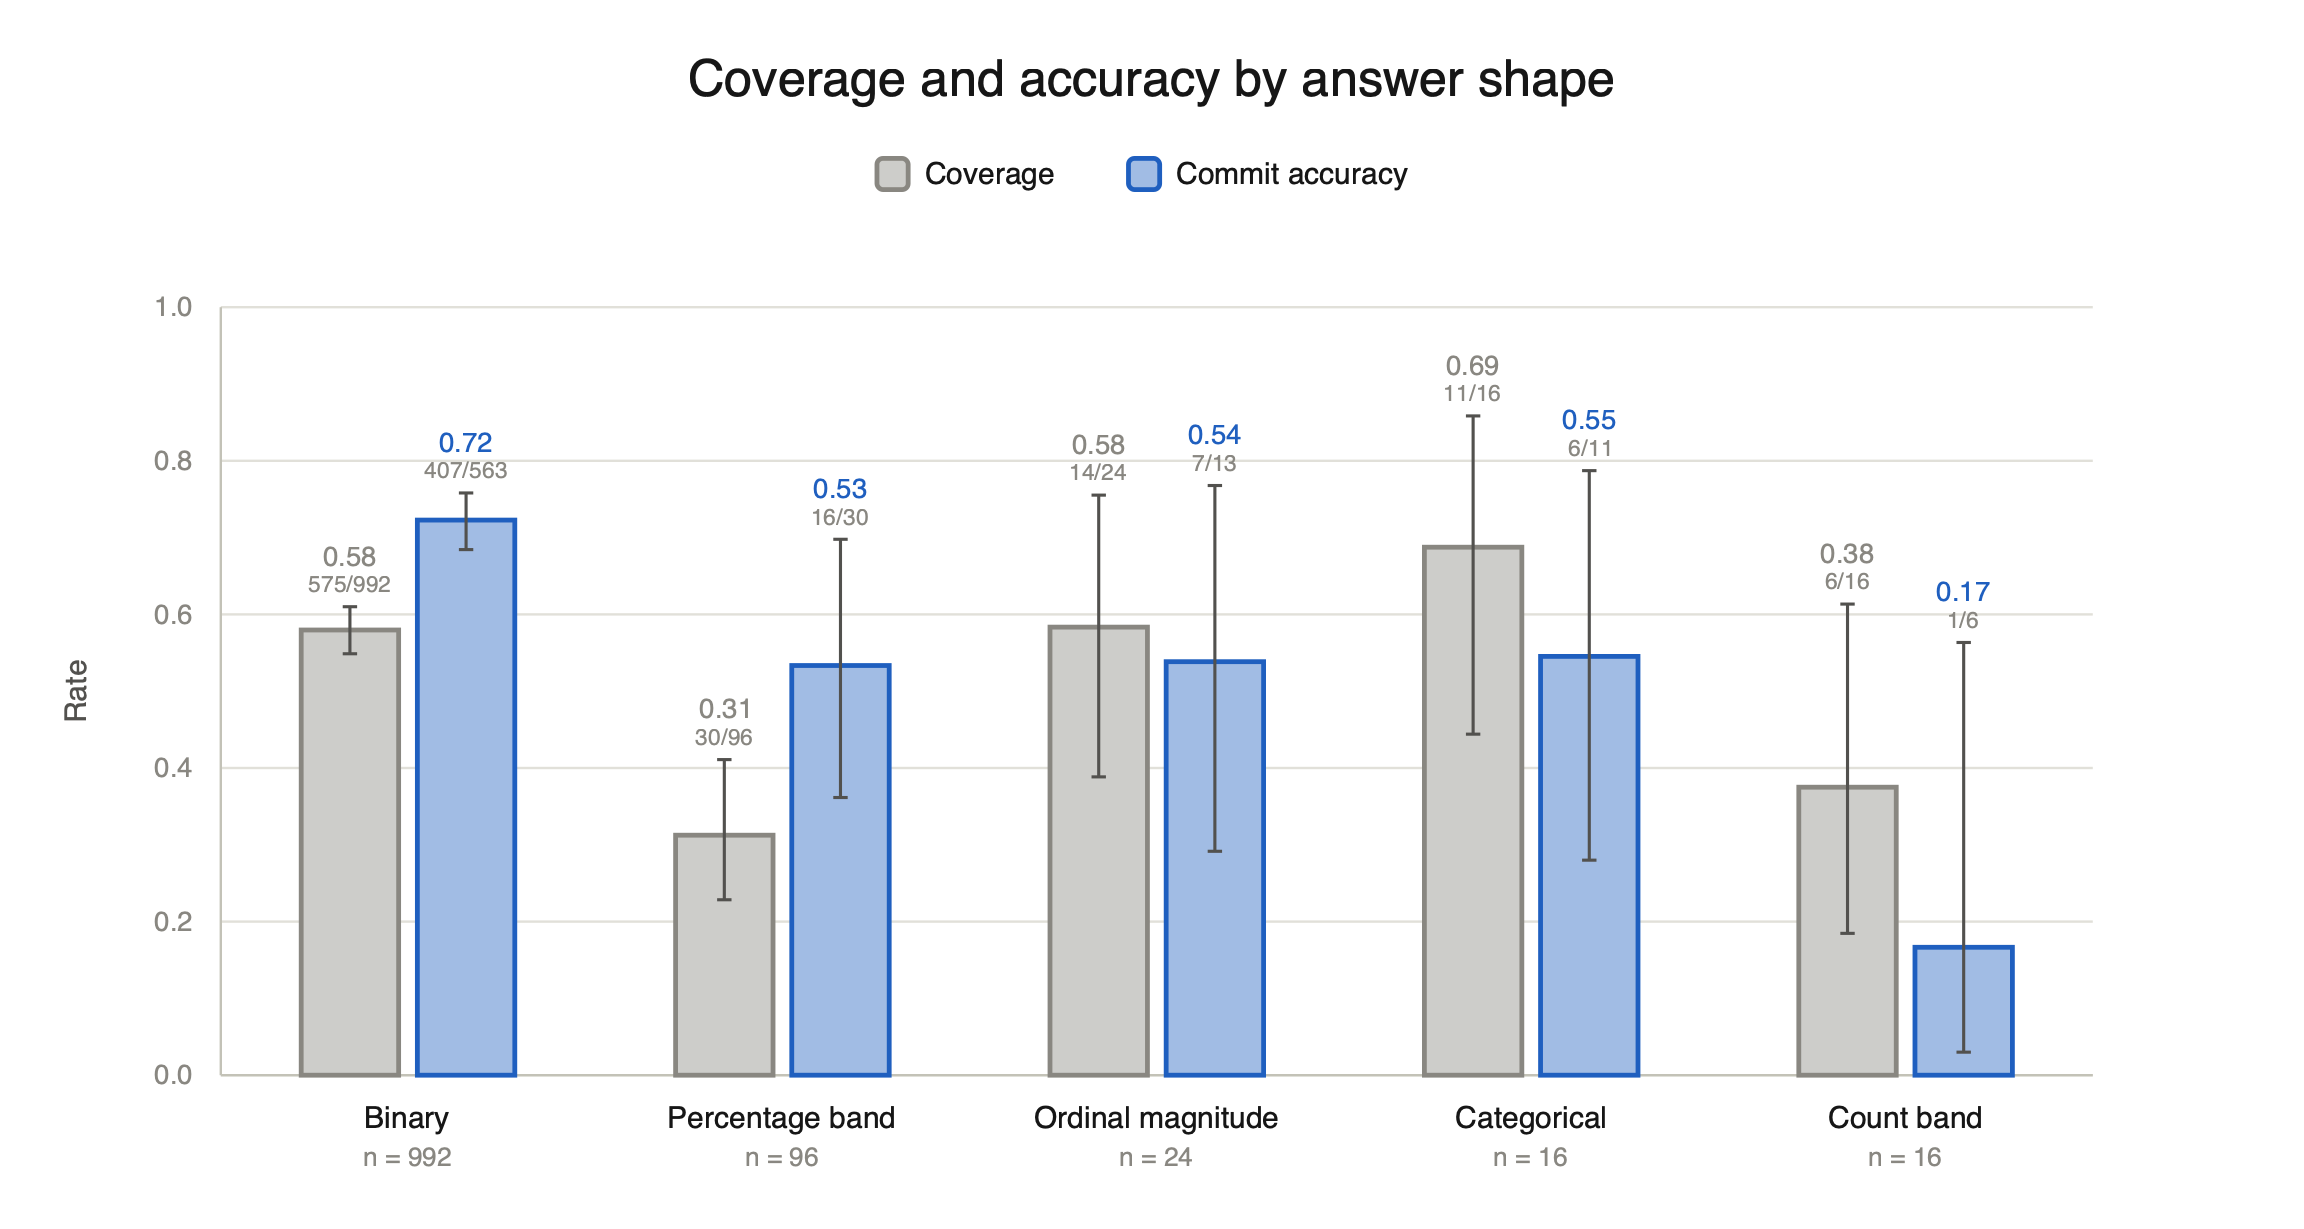
\includegraphics[width=\linewidth]{figures/coverage_accuracy_by_answer_shape.png}
\caption{Coverage and accuracy by answer shape.}
\label{fig:by-answer-shape}
\end{figure}

The spread by answer shape is wider, shown in Figure~\ref{fig:by-answer-shape}, with the nine computable Quality questions set aside. Binary question-country pairs reach 72.3\% commit-accuracy across 992 pairs. The four percentage-band questions outside that set, which ask for a proportion read off a web page, are declined on all 32 of their pairs, and the swarm gets 1 of the 16 count-band questions exactly right. The two shapes it attempts with any regularity, ordinal-magnitude and categorical, reach 29.2\% and 37.5\% over all their pairs, on only 24 and 16 pairs. The majority of what the questionnaire asks in a graded form is either declined or wrong.

Coverage and accuracy must be considered together, because a dimension that abstains from most questions can still achieve a high score on the few it retains. Section~\ref{sec:llm-limitations} set out why an agent constrained to reason from retrieved evidence would fail by over-interpretation, the system attributing evidence that may be adjacent, partial or ambiguous as proof. What varies across the assessment, affecting dimensions and countries alike, is the amount of evidence needed to prove a claim. Portal is the dimension where evidence is dispositive, since a portal feature is either present on the portal or it is not, and Portal is accordingly the strongest of the four on both accuracy and false positives. Policy is the dimension where evidence is abundant and rarely dispositive, since a draft strategy, an EU obligation or a regional initiative all resemble the national instrument the question asks about, and Policy commits most readily and returns a wrong yes on half of all its negative golds. Quality is the dimension where little evidence of any kind reaches the open web, and it declines most and stays second-cleanest on negatives. This is the ordering Section~\ref{sec:subgroup-equity} found across countries rather than questions. Finland, at 77.9 maturity, carries the highest false-positive rate in the run, and Bosnia and Herzegovina, at 15.1, the lowest. A mature country and a Policy question share a property, both hold a significant amount of published material that sits near the question without answering it. Section~\ref{sec:selectivity} shows the same asymmetry at the level of a single answer, where a ``yes'' needs a document and a ``no'' needs an absence that cannot be quoted. The system does not fail where evidence is scarce so much as where evidence is plentiful and beside the point.

\section{Reproducibility}\label{sec:reproducibility}

Reproducibility asks whether the same assessment, run again, returns the same answers. Section~\ref{sec:criteria} set two conditions: a record complete enough for the run to be repeated, covering the prompts issued, the evidence retrieved, the model version and the settings it ran under, and evidence that a repeat returns the same answers. The second matters most for a generative assessor, whose output varies across runs of the same prompt, where the score a country receives should depend only on its data openness.

The first condition holds with one gap. Every Researcher, Verifier and Adjudicator call writes a row carrying the prompt version, the snippets the Researcher read, the model version and the settings. The snippet picker, the model call that selects which passages from each fetched page reach the Researcher, writes no equivalent row for this run, so its prompt and model version sit outside the record. Its output is kept, since the picked snippets are stored against the Researcher call that used them, and the run therefore replays from the Researcher\textquotesingle s inputs onward rather than from every model call. The second condition must be measured between runs, to assess the stability of the answers.

\begin{longtable}[]{@{}
  >{\raggedright\arraybackslash}p{(\linewidth - 10\tabcolsep) * \real{0.1280}}
  >{\raggedright\arraybackslash}p{(\linewidth - 10\tabcolsep) * \real{0.1379}}
  >{\raggedright\arraybackslash}p{(\linewidth - 10\tabcolsep) * \real{0.1477}}
  >{\raggedright\arraybackslash}p{(\linewidth - 10\tabcolsep) * \real{0.1379}}
  >{\raggedright\arraybackslash}p{(\linewidth - 10\tabcolsep) * \real{0.1879}}
  >{\raggedright\arraybackslash}p{(\linewidth - 10\tabcolsep) * \real{0.2094}}@{}}
\caption{The three replicate runs.}\label{tab:replicates}\\
\toprule\noalign{}
\begin{minipage}[b]{\linewidth}\centering
\textbf{Replicate}
\end{minipage} & \begin{minipage}[b]{\linewidth}\centering
\textbf{Finalised}
\end{minipage} & \begin{minipage}[b]{\linewidth}\centering
\textbf{Commit rate}
\end{minipage} & \begin{minipage}[b]{\linewidth}\centering
\textbf{Committed}
\end{minipage} & \begin{minipage}[b]{\linewidth}\centering
\textbf{Commit Accuracy}
\end{minipage} & \begin{minipage}[b]{\linewidth}\centering
\textbf{Aggregate Accuracy}
\end{minipage} \\
\midrule\noalign{}
\endfirsthead
\toprule\noalign{}
\begin{minipage}[b]{\linewidth}\centering
\textbf{Replicate}
\end{minipage} & \begin{minipage}[b]{\linewidth}\centering
\textbf{Finalised}
\end{minipage} & \begin{minipage}[b]{\linewidth}\centering
\textbf{Commit rate}
\end{minipage} & \begin{minipage}[b]{\linewidth}\centering
\textbf{Committed}
\end{minipage} & \begin{minipage}[b]{\linewidth}\centering
\textbf{Commit Accuracy}
\end{minipage} & \begin{minipage}[b]{\linewidth}\centering
\textbf{Aggregate Accuracy}
\end{minipage} \\
\midrule\noalign{}
\endhead
\bottomrule\noalign{}
\endlastfoot
Run 1 & 155 / 156 & 46.6\% & 69 & 69.1\% & 31.8\% \\
Run 2 & 154 / 156 & 44.6\% & 66 & 67.7\% & 29.7\% \\
Run 3 & 151 / 156 & 50.0\% & 74 & 68.5\% & 33.8\% \\
\end{longtable}


Three fresh dispatches of the swarm ran over the 156-pair development battery, with nothing seeded or replayed and the search cache purged before each run, so every replicate found its evidence from scratch. Table~\ref{tab:replicates} gives each run; the eight pairs between the runs that didn't finalise were search stalls, disclosed and excluded, so the analysis rests on the 148 pairs present in all three.

The decision to answer is the unstable part of the system and the answer itself is stable. All three runs reached the same outcome on 70.3\% of the 148 pairs. Commit accuracy moves across a range of 1.4 points while roughly 30\% of pairs change outcome between runs, so disagreements at the level of individual questions largely cancel once they are pooled into a rate. So the official maturity score a country receives may be stable between runs, with a third of underlying evidence varying.

The asymmetry between the two gold classes sits entirely in the decision to answer. Outcome unanimity is 60.5\% on negative golds against 80.0\% on positive ones. The higher variance in negative golds reflects the clustering near and below the confidence threshold from Section~\ref{sec:selectivity}, and pairs that changed outcome between the runs had a median confidence of 0.68, with 44.6\% of them sitting exactly at 0.65. These sparse-evidence pairs are more likely to drop below the threshold than the well-evidenced ``yesses'' that hold between runs. Once all three replicates commit they agree on the label on 47 of 51 pairs, 92.2\%, and that rate holds within both gold classes. What varies with the evidence available is whether the system answers, not the answer it gives.



\begin{figure}[htbp]
\centering
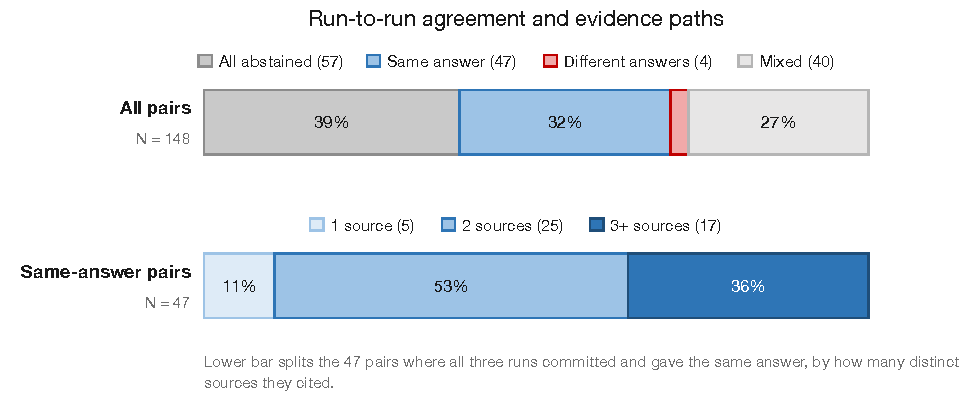
\includegraphics[width=\linewidth]{figures/fig_4_7_1_runtorun.pdf}
\caption{Outcome agreement across the three replicate runs, and the distinct sources cited on the pairs where all three agreed.}
\label{fig:replicates-fig}
\end{figure}

The route to those answers varied far more than the answers did, as the lower bar of Figure~\ref{fig:replicates-fig} shows. Of the 47 pairs where all three replicates committed and agreed, 42 cite two or more distinct source URLs across the runs and 17 cite three. Section~\ref{sec:criteria} anticipated this, that a generative assessor finding its own evidence may issue different queries and read different pages between runs when the underlying truth has not changed, and that what has to hold is the outcome whatever route the model took to it.

Against the two conditions of Section~\ref{sec:criteria}, the record replays and the published score is stable, but the individual question decisions are not. The instability is in whether the system answers a given question at all, and it falls on the thin-evidence negative golds whose confidence sits at the 0.65 floor, where a small shift between runs tips the decision either way. This does not reach the score. A country\textquotesingle s score pools 143 questions, the per-question flips offset each other, and commit accuracy moves only 1.4 points across the three runs. So the number the ODMI would publish is reproducible, but the stability of the evidence for each question varies.

\section{Ablation}\label{sec:ablation}

Each component of the swarm was removed in turn to test what it contributes. The ablation runs on the eight evaluation countries, and four arms are compared. The Researcher alone commits when its own confidence is sufficient, with no second call. The second arm adds the Adversarial Verifier and its retry loop, committing only where the two agents agree within three retries. The third is the full swarm, with the Adjudicator arbitrating disagreements. The fourth replaces the Adversarial Verifier with a corroborative one, prompted to find evidence supporting the Researcher\textquotesingle s claim rather than against it. This arm has no adjudicator, both because a corroborative check produces at most an absence of support rather than a counterargument to weigh, and because the arm exists to isolate the Verifier\textquotesingle s stance.

\begin{longtable}[]{@{}
  >{\raggedright\arraybackslash}p{(\linewidth - 10\tabcolsep) * \real{0.2183}}
  >{\raggedright\arraybackslash}p{(\linewidth - 10\tabcolsep) * \real{0.1776}}
  >{\raggedright\arraybackslash}p{(\linewidth - 10\tabcolsep) * \real{0.1776}}
  >{\raggedright\arraybackslash}p{(\linewidth - 10\tabcolsep) * \real{0.1929}}
  >{\raggedright\arraybackslash}p{(\linewidth - 10\tabcolsep) * \real{0.1269}}
  >{\raggedright\arraybackslash}p{(\linewidth - 10\tabcolsep) * \real{0.1066}}@{}}
\caption{The ablation ladder. Four arms over the 1,144 evaluation pairs, Sonnet 4.6.}\label{tab:ablation}\\
\toprule\noalign{}
\begin{minipage}[b]{\linewidth}\raggedright
\textbf{Configuration}
\end{minipage} & \begin{minipage}[b]{\linewidth}\raggedright
\textbf{Commit rate}
\end{minipage} & \begin{minipage}[b]{\linewidth}\raggedright
\textbf{Commit accuracy}
\end{minipage} & \begin{minipage}[b]{\linewidth}\raggedright
\textbf{Negative-gold FP rate}
\end{minipage} & \begin{minipage}[b]{\linewidth}\raggedright
\textbf{Balanced acc.}
\end{minipage} & \begin{minipage}[b]{\linewidth}\raggedright
\textbf{Youden J}
\end{minipage} \\
\midrule\noalign{}
\endfirsthead
\toprule\noalign{}
\begin{minipage}[b]{\linewidth}\raggedright
\textbf{Configuration}
\end{minipage} & \begin{minipage}[b]{\linewidth}\raggedright
\textbf{Commit rate}
\end{minipage} & \begin{minipage}[b]{\linewidth}\raggedright
\textbf{Commit accuracy}
\end{minipage} & \begin{minipage}[b]{\linewidth}\raggedright
\textbf{Negative-gold FP rate}
\end{minipage} & \begin{minipage}[b]{\linewidth}\raggedright
\textbf{Balanced acc.}
\end{minipage} & \begin{minipage}[b]{\linewidth}\raggedright
\textbf{Youden J}
\end{minipage} \\
\midrule\noalign{}
\endhead
\bottomrule\noalign{}
\endlastfoot
Closed book (no retrieval) & 75.6\% (865/1144) & 55.3\% (476/860) & 13.9\% (51/368) & 0.429 & -0.143 \\
Researcher alone & 26.6\% (304/1144) & 74.3\% (220/296) & 12.5\% (46/368) & 0.173 & -0.653 \\
+ adversarial Verifier & 46.0\% (526/1144) & 72.5\% (372/513) & 23.4\% (86/368) & 0.315 & -0.370 \\
+ Adjudicator (full trio) & 55.6\% (636/1144) & 70.1\% (437/623) & 24.7\% (91/368) & 0.396 & -0.208 \\
Corroborative Verifier & 47.6\% (545/1144) & 71.2\% (380/534) & 27.2\% (100/368) & 0.316 & -0.368 \\
\end{longtable}


Table~\ref{tab:ablation} shows the results of this ablation ladder, covering commit rate, accuracy and negative-gold false-positive rate. The headline result is the improvement in coverage rather than raw accuracy. The Researcher alone commits on 26.6\% of the pairs, lifting to 46.0\% with the Adversarial Verifier and 55.6\% with the Adjudicator. The number of correct answers rises with it, from 220 to 372 to 437 out of 1,144. The Verifier turns 165 of the Researcher\textquotesingle s wrong or withheld answers into correct ones and loses 13 the other way, and the Adjudicator adds 65 correct answers while reversing none.

Accuracy on the answers each arm keeps moves the other way. The Researcher alone reproduces the published key on 74.3\% of what it commits, the Adversarial Verifier arm on 72.5\%, and the full trio on 70.1\%. The closed-book floor commits readily, on 75.6\% of pairs, and reproduces the key on 55.3\% of them, so the evidence the swarm gathers is worth fifteen points of commit accuracy over the model\textquotesingle s own priors.

That gap closes once both are made to answer everything. Scoring every binary question and counting a declined one as wrong, the closed-book model reproduces 43.0\% of the key and the full swarm 42.4\%. Retrieval does not raise the number of questions the system gets right. It raises the share it gets right among the ones it keeps, which is a claim about selection and not about knowledge.

Two results complicate this picture. The first is that the Adversarial Verifier does not filter for precision. If it did, it would commit fewer wrong answers on the negative golds than the Researcher alone. It commits more. Coverage rises from 26.6\% to 46.0\% and the false-positive rate climbs with it, from 12.5\% to 23.4\%. The Adjudicator raises coverage again to 55.6\%, adding five further wrong commitments on the negative golds and recovering none, which leaves the rate almost unmoved at 24.7\%. That it costs so little supports Tyen et al.\textquotesingle s finding that a model rules on a located error far more reliably than it detects one unaided, since the Adjudicator only ever sees a disagreement the Verifier has already drawn. The closed-book floor puts the problem at its sharpest. Answering from its parameters alone, it asserts a wrong yes on 13.9\% of the negative golds against the full trio\textquotesingle s 24.7\%, so a model with no evidence in front of it commits fewer false yeses than the architecture built to prevent them.

The obvious objection is that the closed-book model only looks precise because it declines more of the hard questions. It does not. It commits on 56.8\% of the negative golds where the full swarm commits on 50.0\%, so it answers more of them and still recovers 42.1\% of the no answers against the swarm\textquotesingle s 24.5\%. Searching the web nearly halves the system\textquotesingle s ability to establish that a practice is absent. The likely reason is what a search returns. Material adjacent to a practice reads as evidence that the practice exists, and nothing comes back that evidences its absence. This comparison cannot prove that on its own, since the closed-book arm differs from the Researcher in its prompt, its lack of a confidence gate and its lack of a Verifier, so a readier disposition to answer ``no'' is not ruled out.

The two are also right about different questions. Across the binary golds they agree on 243 and disagree on 289, with 142 going to the swarm and 147 to the closed-book model, at a McNemar p of 0.8140. A system able to pick the better of the two on each question would reach 58.7\%, well above either alone. Retrieval and parametric recall are close to independent here, which this design was not built to exploit.

The second result is that the Verifier\textquotesingle s stance does not matter. Swapping the Verifier from adversarial to corroborative changes very little. Balanced accuracy moves from 31.5\% to 31.6\%. Of the 110 pairs one arm answered correctly and the other did not, 51 went to the adversarial arm and 59 to the corroborative, at a McNemar p of 0.5047. On total accuracy, which counts an abstention as a miss, the arms sit at 32.5\% and 33.2\%, a difference of 0.7 points against a paired standard error of 0.9, and this is evidence of equivalence. Section~\ref{sec:verification-methods} and Section~\ref{sec:debate} argue that opposition succeeds where corroboration fails in a thin-evidence setting, because corroboration compounds the model\textquotesingle s guessing bias while refutation checks it. On accuracy that argument is not supported.

It survives on the negative golds, where the adversarial arm commits a wrong answer on 23.4\% against the corroborative arm\textquotesingle s 27.2\%, and of the 50 where exactly one arm went wrong, 32 came from the corroborative arm, at p of 0.0649. Corroboration raises yes-recall from 52.1\% to 55.8\% and lowers no-recall from 10.9\% to 7.3\%, the guessing bias Section~\ref{sec:debate} describes, short of significance.

The literature anticipates this. \textcite{chowdhury2026} assign a different model to each of their judges, on the argument that agents drawn from the same weights cannot be relied on to disagree. Their own ablation locates the largest single gain not in the argumentation structure but in progressive evidence retrieval, 7.5 points of their 10.0-point improvement over standard multi-agent debate. \textcite{zhu2026} attribute the benefit of debate to agent diversity rather than to the framework itself. Here the Researcher and Verifier are the same Claude model, so the change in stance is a prompt difference and nothing more, and a prompt difference producing an equivalence result is what this literature would predict.

Both halves point the same way, and it is the conclusion Section~\ref{sec:selectivity} and Section~\ref{sec:attributability} reach from other directions, that every mechanism built to control precision acted on coverage instead.

\section{Operational Cost and Runtime}\label{sec:cost-runtime}

Section~\ref{sec:criteria} set timeliness and cost-effectiveness aside from the six criteria, since neither addresses whether the automation upheld the legitimacy previously assumed by the human rater. Both still matter for whether automation is worth running at all, given the labour a 5,148-question assessment demands.

One caveat governs every figure below. The system runs through a local proxy against a flat subscription, so the marginal cost of a run is zero and the sterling amounts are notional, converting logged tokens at published list prices to give what the same work would cost on a metered API. The figures cover every model call the pipeline makes. The three agents account for 23\% of the spend, the remaining 77\% goes to the snippet picker, the call that reads each fetched page and selects the passages the Researcher reasons over (Section~\ref{sec:retrieval}). The system spends over three times as much reading pages as it does reasoning about what it read.

Answering all 1,144 evaluation pairs cost £375 in notional compute, spread across the denominators of Table~\ref{tab:cost}: £0.33 per attempted pair, £0.59 per answer given, and £0.86 per answer that matched the key, of which there were 437.

\begin{longtable}[]{@{}
  >{\raggedright\arraybackslash}p{(\linewidth - 4\tabcolsep) * \real{0.5556}}
  >{\raggedright\arraybackslash}p{(\linewidth - 4\tabcolsep) * \real{0.1944}}
  >{\raggedright\arraybackslash}p{(\linewidth - 4\tabcolsep) * \real{0.2500}}@{}}
\caption{What the assessment cost.}\label{tab:cost}\\
\toprule\noalign{}
\begin{minipage}[b]{\linewidth}\raggedright
\textbf{Basis}
\end{minipage} & \begin{minipage}[b]{\linewidth}\raggedright
\textbf{Pairs}
\end{minipage} & \begin{minipage}[b]{\linewidth}\raggedright
\textbf{Cost per pair}
\end{minipage} \\
\midrule\noalign{}
\endfirsthead
\toprule\noalign{}
\begin{minipage}[b]{\linewidth}\raggedright
\textbf{Basis}
\end{minipage} & \begin{minipage}[b]{\linewidth}\raggedright
\textbf{Pairs}
\end{minipage} & \begin{minipage}[b]{\linewidth}\raggedright
\textbf{Cost per pair}
\end{minipage} \\
\midrule\noalign{}
\endhead
\bottomrule\noalign{}
\endlastfoot
Every pair attempted & 1,144 & £0.33 \\
Pairs the swarm answered & 636 & £0.59 \\
Answers matching the key & 437 & £0.86 \\
A pair it committed to & 636 & £0.28 \\
A pair it abstained on & 508 & £0.41 \\
Whole evaluation run & 1,144 & £375 total \\
\end{longtable}


These figures are averages; pair cost varies with the number of calls required. A pair that the system committed to cost £0.26 and required 2.2 attempts, whereas a pair on which it abstained cost £0.41 and used the full three-retry budget, because under the loop described in Section~\ref{sec:agent-loop} a pair reaches abstention only after all retries are exhausted. Section~\ref{sec:selectivity} argued that abstention is the honest outcome when evidence is thin, and this is the cost of that honesty. Selectivity is the most expensive result for a pair.

Per-country cost is nearly flat, from £0.310 in Finland to £0.348 in Bosnia and Herzegovina, up to £0.385 with Bulgaria, and most of that spread is the abstention mix rather than anything about how hard a country\textquotesingle s evidence is to read. Bosnia abstains on 61.5\% of its pairs against Finland\textquotesingle s 25.9\%, and an abstained pair costs 58\% more than a committed one does. Set against Section~\ref{sec:subgroup-equity}, where coverage, commit accuracy and the false-positive rate all track published maturity, cost is the one measure that does not.\textbf{ }

Model choice is the other lever, and Appendix~\ref{app:experiments} gives the comparison across Haiku 4.5, Sonnet 4.6 and Opus 4.8 on the development battery. It moves how much the system is willing to say, rather than how often it is right. Sonnet is retained because it commits most, at a middling price, with commit-accuracy indistinguishable from Opus, which costs over three times as much.

A pair took a median of 200 seconds from its first logged Researcher call to its finalised row, counting the searches issued and the pages fetched alongside the model\textquotesingle s own work, and 95\% finished inside six minutes. This is an upper bound under load, since up to twenty pairs ran simultaneously on one machine competing for the same connection. Three pairs ran past thirty minutes, the longest at forty-nine, each stalled on an unresponsive server with the Swedish catalogue endpoint worst among them.

The eight evaluation countries took 45 hours and £375, so all 36 extrapolate to roughly 200 hours and £1,700. The time is an upper bound, since the eight were chosen to oversample negative golds, which skews them below the European average on maturity, and Section~\ref{sec:subgroup-equity} found lower-maturity countries abstain more, sending more pairs through the full retry budget.

This £1,700 does not buy a completed assessment, as the coverage across the eight countries is 55.6\%. The system would commit to around 2,860 of the 5,148 pairs and decline the other 2,290. Of the answers it commits to, 70.1\% match the published key. In practice, if this system ran as a precursor to human judgement, an assessor following it would have two populations to work on. The 2,290 declined pairs arrive as a visible queue, flagged and easy to route. The harder population is the 850 or so committed answers that are wrong, which look ostensibly identical to the correct answers, with the same structure of quote and source as the 2,010 that are right.

\section{Reconstructing the Index}\label{sec:reconstruction}

The point of this exercise is to see whether a human-labour-intensive process could be replaced by an automated one. This section constructs what the maturity score would be across the eight evaluation countries, and what work would be left for the humans overseeing the automation.

The ODMI computes each country\textquotesingle s score as the unweighted mean of four dimension percentages, each the marks awarded across its questions divided by the marks available. The rubric is not published but is recoverable from the answer key, at 345 distinct answer-to-score mappings across the 143 questions. Applying it to the published answers reproduces the 2025 figures exactly, at 100.0 for France and 62.9 for Bulgaria, which establishes that the recovered rubric reconstructs the ODMI\textquotesingle s arithmetic. Where the swarm returns an answer the rubric does not recognise, that answer scores zero.

Abstention makes the result a range rather than a figure. The floor scores every abstention as zero, and represents what a country could be awarded on public evidence alone. The ceiling scores only the pairs the swarm committed to, so it assumes the declined pairs would have scored at the same rate. That is optimistic, since Section~\ref{sec:selectivity} showed the swarm abstains on the questions it finds hardest.



\begin{figure}[htbp]
\centering
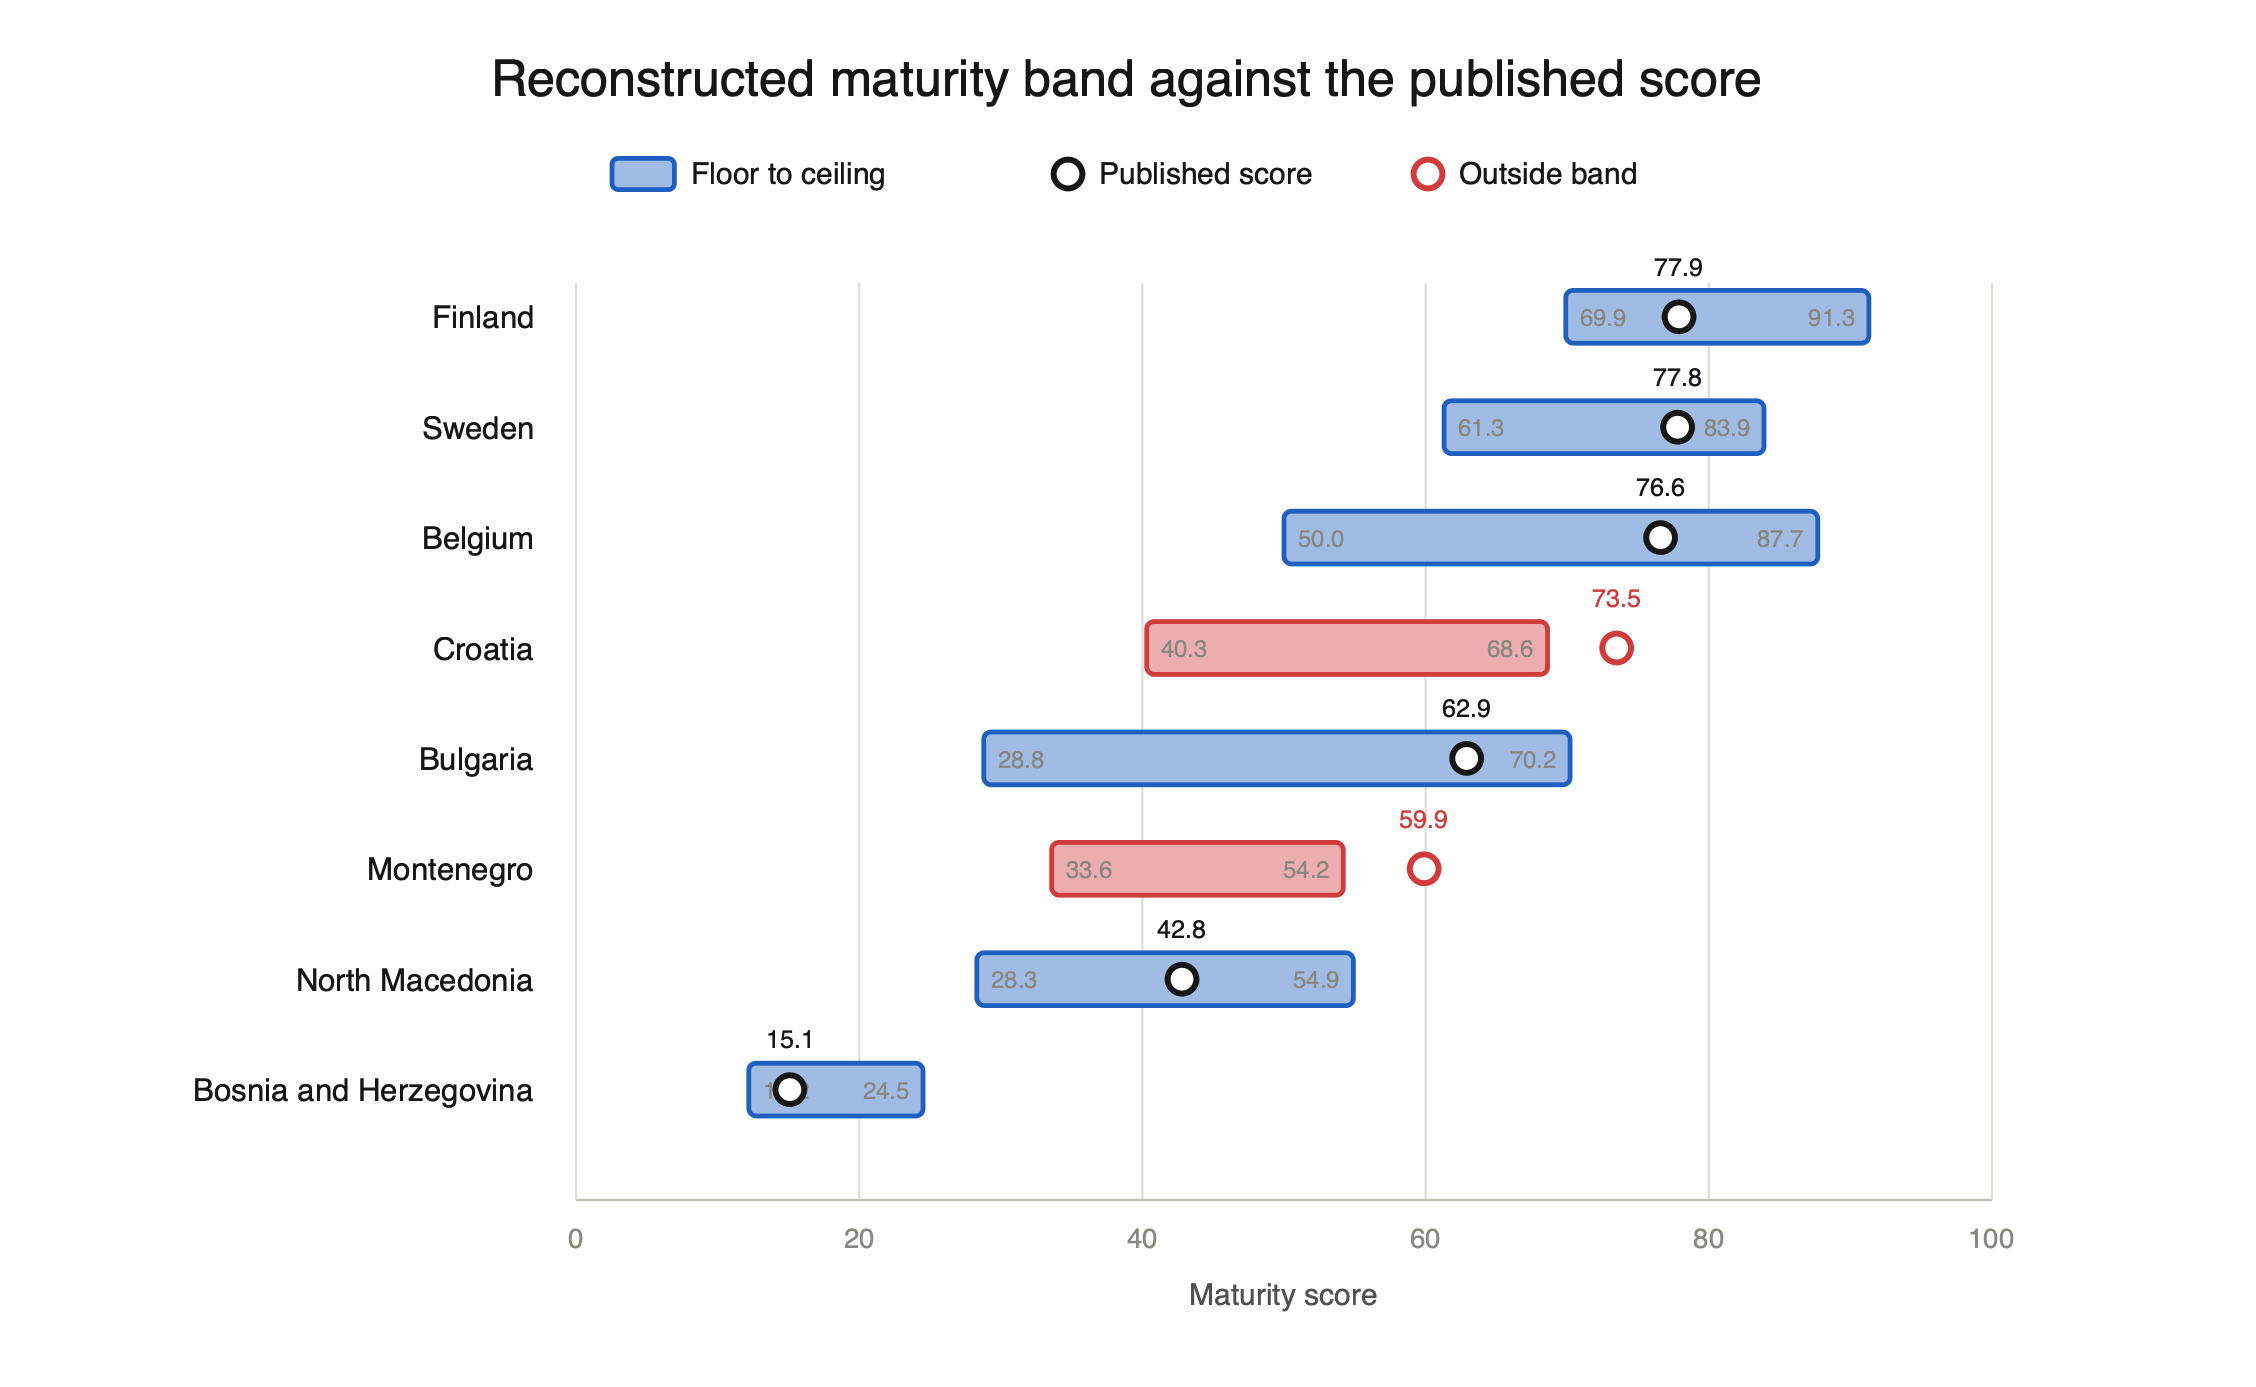
\includegraphics[width=\linewidth]{figures/reconstructed_band.png}
\caption{Reconstructed maturity band against the published score.}
\label{fig:reconstruction-fig}
\end{figure}

Ranking the eight by their reconstructed ceiling and comparing to the published order gives a Spearman correlation of 0.929, and on the floor 0.976. Section~\ref{sec:subgroup-equity} found coverage tracking published maturity at ρ = 0.81, and the floor is depressed by abstention, so a low-maturity country is pushed down the floor ordering by declining more as well as by scoring less. The ceiling removes that effect, since it divides only by what the swarm attempted. Per-country commit accuracy ranges from 52.8\% to 82.1\% and coverage from 38.5\% to 74.1\%, so there was ample room for the ordering to scramble, and yet it largely survived. The mean band spans 26.4 points and the published score falls inside it for six of the eight countries, as Figure~\ref{fig:reconstruction-fig} shows.

Two countries fall outside their band, and in the same direction. Croatia\textquotesingle s published 73.5 sits above a ceiling of 68.6, and Montenegro\textquotesingle s 59.9 above a ceiling of 54.2. In both cases the swarm cannot reach the published figure even crediting every declined question as though it had performed like the ones the swarm answered.

The ODMI states four purposes for the assessment: to help a country understand its own maturity, to capture its progress year on year, to identify areas for improvement, and to benchmark its performance against other countries. Benchmarking is recovered, as the swarm orders the eight countries almost exactly as the assessors do, and it does so on public evidence alone.

Understanding their own maturity is partly recovered. Where the swarm commits, it agrees with the published answer 70.1\% of the time, so a country reading the individual answers gets a substantially accurate picture of what an external assessor found. However, aggregating 143 of those into a single figure is where the precision goes, and the 26-point average band shows this.

Identifying areas for improvement depends on which area. Section~\ref{sec:generalisability} found the swarm reliable on Portal, at 78.4\% commit accuracy with a 13.2\% false-positive rate, so a Portal shortfall is worth acting on. Policy is the reverse: it commits most readily and returns a wrong yes on half its negative golds, so a Policy pass carries little information. A country acting on this output would need the per-dimension reliability published alongside it.

Year-on-year progress is out of reach on two counts. A country typically moves a few points a cycle, well inside a 26-point band, and Section~\ref{sec:reproducibility} found the per-question decision unstable across runs, so a difference between two cycles would carry sampling variation alongside real change.

The nine sections above describe one constraint. The swarm reproduces the published key on 70.1\% of the answers it commits to, against 43\% for the same model with no retrieval at all, and it reaches that figure by declining 44\% of the questions. Forced to answer everything, it falls below a blanket yes. The system declines half the questions whose answer is no against 37.1\% of those whose answer is yes, and each criterion above records a different consequence of that. Confidence measures how easy a claim was to evidence rather than how likely it is to hold. The two mechanisms built to control precision both acted on coverage. The error rises with a country\textquotesingle s published maturity, so it tracks the quantity the index exists to estimate. The searches themselves worked, and no abstention in this run came from an empty search. The system found material and could not turn it into evidence of an absence. Chapter~\ref{ch:discussion} takes up what would have to change, in the architecture and in the questionnaire, for a ``no'' to be evidenced on the same terms as a ``yes''.
